%  Typ dokumentu - článek, prezentace aj.
\documentclass[english]{article}

%  Nastaví vstupní a výstupní kódování znaků (encoding) a lokalizace
\usepackage[T1]{fontenc}
\usepackage[utf8]{inputenc}
\usepackage[english,czech]{babel}
\usepackage{icomma}
\usepackage{lmodern}

%  Formát papíru a odsazení od jeho okrajů
\usepackage[letterpaper]{geometry}
\geometry{verbose,tmargin=1.5cm,bmargin=2cm,lmargin=2cm,rmargin=2cm}

%  Umožňuje pracovat s grafikou
\usepackage{graphicx}
\usepackage{bigstrut}

%  Automaticky odsadí i první paragraf v každé sekci
\usepackage{indentfirst}

%  Umožňuje rozdělovat obsah na více sloupců
\usepackage{multicol}
\usepackage{booktabs}

%  Umožňuje používat hypertextové odkazy, nastavuje jejich barvu a
%  vlastnosti
\usepackage[unicode]{hyperref}
\hypersetup{
colorlinks=true, citecolor=blue, filecolor=blue, linkcolor=blue,
urlcolor=blue
}

%  Umožnění odstranění italiky u jednotek
\newcommand{\unit}[1]{\mathrm{#1}}

%  Formátování stránek, empty = odstraní číslování
% \pagestyle{empty}

%  Řádkování
\linespread{1.2}

%  Lepší zobrazování matematiky (rozšíření sum o \limits atd.)
\everymath{\displaystyle}
\usepackage{amsmath, amsthm, amssymb}

% Umožní psát přes \mathbb{N/R/Q/..} množiny čísel
\usepackage{amssymb}

%  Velikost fontu matematických výrazů v dokumentu lze pro danou
% základního fontu dokumentu upravit pomocí:
% \DeclareMathSizes{X}{Y}{Z}{U} kde:
% X je velikost fontu v dokumentu, pro kterou se matematika upraví
% Y je standartní velikost fontu matematiky
% Z je velikost fontu zmenšených (vnořených výrazů)
% U je velikost fontu ještě více zmenšených (vnořených výrazů).
\DeclareMathSizes{10}{10.5}{9}{9}

%  Nastaví autora, název, datum, skupinu měření apod. (můj vlastní
% příkaz, umožní znovu-použití v dokumentu)
\newcommand{\Author}{David Roesel}
\newcommand{\Coauthor}{Tereza Schönfeldová}
\newcommand{\Institute}{FJFI ČVUT v Praze}
\newcommand{\Subject}{FYZIKÁLNÍ PRAKTIKUM I}
\newcommand{\Group}{7}
\newcommand{\Circle}{ZS 5}
\newcommand{\Title}{Úloha \#2  \\Měření modulu pružnosti v tahu \\ a modulu pružnosti ve smyku}
\newcommand{\Date}{22.11.2013}

% Začátek dokumentu - Formátování na výstup
\begin{document}

% Interní proměnné, možno zobrazovat u prezentací, používají se při
% generování pomocí \titlepage apod.
\author{\Author}
\title{\Title}
\date{\Date}

%  Lokalizace některých názvů do češtiny
\renewcommand{\figurename}{Obr.}
\renewcommand{\tablename}{Tab.}
\renewcommand{\refname}{Reference}

% --- Hlavička dokumentu -----------------------------------------------

\setlength{\parindent}{0cm}
\begin{multicols}{2}
\textbf{\Subject \\
        \Institute \\[0.1cm]
%\large  \Title \\[0.5cm]
\Title \\[0.5cm]
}
\begin{tabular}{rlrl}
\large Datum měření: & \Date & \large Skupina: & \Group \\
\large Jméno: & \Author & \large Kroužek:  & \Circle\\
\large Spolupracovala: & \Coauthor &\large Klasifikace:\\
\end{tabular}

\begin{flushright}

\includegraphics[scale=0.28]{../../_meta/fjfi_standart.pdf}
\hspace{0.2cm}
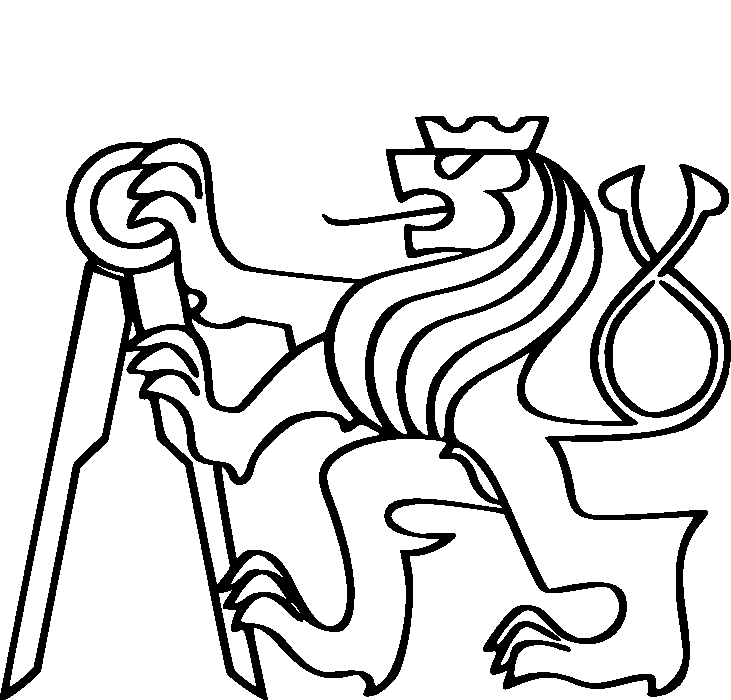
\includegraphics[scale=0.28]{../../_meta/cvut_standart.pdf}
\end{flushright}
\end{multicols}
\hrule
\vspace{0.5cm}

% ----------------------------------------------------------------------


% --- Tělo dokumentu ---------------------------------------------------
\setlength{\parindent}{0.5cm}

\section{Pracovní úkoly}
		\begin{enumerate}
		\item Změřte závislost relativního délkového prodloužení $\Delta l / l$ ocelového drátu na napětí při zatěžování a odlehčování drátu a sestrojte graf této závislosti. Vypočítejte metodou nejmenších čtverců modul pružnosti v tahu ocelového drátu.
		\item Změřte závislost průhybu $z$ na velikosti síly $F$ při zatěžování i odlehčování ocelového nosníku a narýsujte graf této závislosti. Metodou nejmenších čtverců vypočítejte modul pružnosti v tahu. O způsobu zpracování výsledků metodou nejmenších čtverců se dočtete v příloze dokumentu \cite{bib:zadani}.
		\item V přípravě odvoďte vzorec pro plošný moment setrvačnosti obdélníkového průřezu šířky $a$ a výšky $b$.
		\item Změřte závislost úhlu zkroucení $\varphi$ ocelového drátu na velikosti kroutícího momentu při postupném zvětšování a postupném zmenšování tohoto momentu. Výsledky měření vyneste do grafu. Metodou nejmenších čtverců vypočtěte modul pružnosti ve smyku $G$ drátu.
		\item Na torzním kyvadle změřte moment setrvačnosti základního systému $I_0$ a modul pružnosti ve smyku $G$ ocelového drátu. Dobu torzních kmitů změřte postupnou metodou.
		\item V přípravě odvoďte vzorce pro výpočet modulu pružnosti ve smyku $G$ a momentu setrvačnosti základního systému torzního kyvadla $I_0$.
		\end{enumerate}
	
\section{Vypracování}

	\subsection{Použité přístroje}
			Stojan s indikátorovými hodinkami a ocelovým drátem, zařízení na měření modulu pružnosti v tahu z průhybu nosníku, zařízení na měření modulu pružnosti ve smyku z torze drátu statickou a dynamickou metodou, mikrometrický šroub, posuvné měřítko, svinovací metr, váhy,  sada závaží, mobilní telefon. 
	
	\subsection{Teoretický úvod}
			
			\subsubsection{Modul pružnosti v tahu a modul pružnosti ve smyku}
					Pružnost homogenního izotropního tělesa popisujeme při malých deformacích dvěma nezávislými materiálovými konstantami, kterými jsou buď \textit{modul pružnosti v tahu} (Youngův modul) $E$ a Poissonovo číslo $\mu$, anebo např. 	\textit{modul pružnosti v tahu} $E$ a \textit{modul pružnosti ve smyku} $G$. 
					
					Uvažujme hranol či válec o průřezu $S$ a délce $l$ s upevněným jedním koncem. Necháme-li ve směru podélné osy působit sílu $F$, vyvolá prodloužení původní délky $l$ o $\Delta l$. Mezi napětím $F/S$ a relativním prodloužením $\Delta l/l$ platí tzv. Hookeův zákon
							\begin{equation} \label{eq:younguv_modul}
							\frac{F}{S} = E \frac{\Delta l }{l}.
							\end{equation}
					Konstanta $E$ závisí na materiálu a nazývá se \textit{modul pružnosti v tahu} (neboli Youngův modul).
					
					Pro druhý případ uvažujme krychli o hraně $l$ z materiálu, jehož vlastnosti chceme zkoumat. Dolní podstavu upevníme a v horní necháme působit sílu $F$ rovnoběžně s dolní podstavou, která horní postavu posune a změní původně pravý úhel o malý úhel $\gamma$ tak jako na Obr. \ref{fig:s_smyk}. Mezi smykovým napětím $F/S$ a smykovou deformací (úhlem smyku $\gamma$) platí pro malé posunutí vztah
							\begin{equation}
							\frac{F}{S} = G \gamma,
							\end{equation}
					kde $G$ je konstanta určená vlastnostmi materiálu a nazývá se \textit{modul pružnosti ve smyku}.
			
			\subsubsection{Ohyb nosníku}
					Uvažujme přímý nosník délky $l$ o průřezu libovolného tvaru ohnutý stejně jako na Obr. \ref{fig:s_ohyb}. Chceme určit vztah mezi rozměry a tvarem nosníku, konstantami charakterizujícími vlastnosti materiálu a mezi silami působícími na nosník. Z Obr. \ref{fig:s_neutralniplocha} můžeme odvodit, že je prodloužení $\Delta l$ úměrné $y$ podle vzorce 
								\begin{equation}
								\frac{\Delta l}{l} = \frac{y}{R},
								\end{equation}
					kde $l$ je délka a $R$ poloměr křivosti nosníku. Stejně tak napětí $\Delta F/\Delta S$ je úměrné $y$ podle vztahu
								\begin{equation} \label{eq:sila_na_plochu_pricny_prurez}
								\frac{\Delta F}{\Delta S} = E \frac{y}{R}.
								\end{equation}	
					Ze stejného obrázku můžeme stanovit pro velikost momentu dvojice sil $M$ vztah
					
					\begin{equation}
					M = \int_{\mathcal{S}} y\ \mathrm{d}F = \frac{E}{R} \int_{\mathcal{S}} y^2\ \mathrm{d}S,
					\end{equation}
				   	kde $S$ je příčný průřez nosníku a integrál na pravé straně nazveme plošným momentem setrvačnosti $I$, jehož velikost jsme pro náš případ (obdélníkový průřez rozměrů $a\cdot b$) v domácí přípravě odvodili následovně:
				   	\begin{equation}
				   	I = \int_{\mathcal{S}}y^2\ \mathrm{d}S = \int_{0}^{a}\int_{-b/2}^{b/2}  y^2\ dxdy = a\int_{-b/2}^{b/2}  y^2 dy = \frac{ab^3}{12}.
				   	\end{equation}
					
					Pro pohybový moment nosníku s pevnými konci, který ohýbáme uprostřed (viz Obr. \ref{fig:s_ohyb_priklad}), platí 
					\begin{equation}
		     		M(x) = \frac{F}{2}\left( \frac{L}{2} - x \right),
					\end{equation}
					kde $F$ je síla působící na nosník v bodě závěsu a $L$ jeho délka.  Kombinací předchozích vztahů dostáváme vztah
					\begin{equation}
					\frac{\mathrm{d}^2z}{\mathrm{d}x^2} = \frac{F}{2EI}\left( \frac{L}{2} - x \right)
					\end{equation}
					a jeho integrací za použití počátečních podmínek ($x = 0$, $dz/dx=0$) a okrajových podmínek ($x=L/2$, $z=0$) pak
					\begin{equation}
					z(x) = \frac{F}{2EI} \left( \frac{Lx^2}{4} - \frac{x^3}{6} \right) - \frac{FL^3}{48 EI},
					\end{equation}
					potažmo (pro průhyb uprostřed nosníku)
					\begin{equation}\label{eq:pruhyb_tyce_ve_stredu}
					z(0) = - \frac{FL^3}{48 EI}.
					\end{equation}
		
			\subsubsection{Torze válce kruhového průřezu}
					Uvažujme válec o délce $L$ a poloměru $R$, jehož horní podstava je upevněna a spodní je vůči ní stočena o úhel $\varphi$ (tak jako na Obr. \ref{fig:torze_valce}). Tuto deformaci nazýváme torze. Pro torzi definujeme veličinu $\alpha$, která se nazývá mírou torze a je to úhel stočení dvou kolmých průřezů vzdálených od sebe o jednotkovou délku. Platí tedy vztah $\varphi = L \alpha$. 
					
					Představme si elementární hranol vyříznutý z válce o délce $r \mathrm{d} \psi$, šířce $\mathrm{d}r$ a výšce $\mathrm{d}l$ (viz Obr. \ref{fig:torze_element}). Tento hranol se při torzi deformuje. Neuvažujeme-li posunutí a otočení kolem podélné osy válce, prodělá každý elementární hranol smyk. Pro hranol vzdálený o $r$ od osy válce je posunutí spodní podstavy vůči horní  $\delta = r \alpha \mathrm{d}l$ a pro úhel smyku $\gamma = \delta/\mathrm{d}l = r \alpha$. Z Obr. \ref{fig:torze_element} vidíme, že pro přírůstek momentu sil $M$ platí	
					\begin{equation}
					\mathrm{d}M = r \frac{F}{S} \mathrm{d}S,
					\end{equation}
					kde $\mathrm{d}S$ je plocha podstavy elementárního hranolu $\mathrm{d}S = r \mathrm{d}\psi \mathrm{d}r$. Celkový moment sil $M$ vyvolávající torzi válce je pak 
					\begin{equation}\label{eq:G_torze}
					M = \int_{0}^{2 \pi}\int_{0}^{R} r \tau \mathrm{d}\psi \mathrm{d}r = G \alpha \int_{0}^{2 \pi}\int_{0}^{R} r^3 \mathrm{d}\psi \mathrm{d}r = G \frac{\pi R^4}{2L}\varphi,
					\end{equation}
					přičemž při tíhovém zrychlení $g$ a poloměru kladky $a$ je pro moment síly dvou závaží o hmotnostech $m_1$ a $m_2$ roven 
					\begin{equation}\label{eq:G_torze2}
					M=(m_1+m_2)ga.
					\end{equation}			
						
			\subsubsection{Torzní kyvadlo}
					Pro tyč torzního kyvadla platí
					\begin{equation}
					I \frac{\mathrm{d}^2 \varphi}{\mathrm{d} t^2} = - K \varphi, \qquad \qquad \qquad K = \frac{G \pi R^4}{2L},
					\end{equation}
					kde $I$ je moment setrvačnosti tyče a na ni přidaných závaží, $\varphi$ úhel torze drátu, $G$ modul pružnosti ve smyku, $t$ čas, $R$ poloměr a $L$ délka drátu. V domácí přípravě jsme odvodili vztah pro modul pružnosti ve smyku $G$ 
					\begin{equation}\label{eq:G_kmity}
							G=\frac{8\pi L I}{T^2R^4}
					\end{equation}			
					a dále víme, že pro moment setrvačnosti $I_v$ dutého válce o vnitřním a vnějším poloměru $r_1$, $r_2$, hmotnosti $m$ a výšce $v$ vzhledem k ose kolmé k ose rotace válce platí při délce ramena tyče $a$
					\begin{equation}\label{eq:teo_steiner}
					I_v = M\cdot (a-\frac{1}{2}v)^2 + \frac{M}{4}(r_1^2 + r_2^2 + \frac{v^2}{3}).
					\end{equation}					
					V domácí přípravě jsme dále odvodili pro momenty setrvačnosti dutých válců $I_1$, $I_2$ umístěných na tyči torzního kyvadla, pro jejich periody $T_1$, $T_2$ a moment setrvačnosti samotné tyče $I_0$
					\begin{equation}
							I_0 = \frac{I_1T_2^2-I_2T_1^2}{T_1^2-T_2^2}.
					\end{equation} 
					Největší přesnosti a nejsnadnějšího výpočtu dosáhneme v případě, že zvolíme za závaží o momentu $I_2$ závaží o nulové hmotnosti (a tím pádem i nulového momentu setrvačnosti). Tím se nám vzorec zjednoduší (při přeznačení $T_2 \rightarrow T_0$) na 
					\begin{equation}\label{eq:I_0}
							I_0 = \frac{I_1T_0^2}{T_1^2-T_0^2}.
					\end{equation} 
					
	\subsection{Postup měření}
			\subsubsection{Měření modulu pružnosti v tahu \emph{E} z prodloužení drátu}
					Modul pružnosti v tahu ocelového drátu jsme měřili přímou metodou z prodloužení $\Delta l$ v závislosti na napínací síle. Drát byl napínán silou $F$ způsobenou vahou závaží, které bylo zavěšené na jeho neupevněném konci. Drát jsme nejdříve napnuli závažím o hmotnosti kolem 1 kg. Následně jsme změřili jeho délku a průměr. Vlastní měření jsme prováděli následovně (s již sestavenou aparaturou):
					\begin{enumerate}
							\item Na háček indikátorových hodinek (nebo na poslední zavěšené závaží) zavěsíme jemně (z důvodu hystereze) závažíčko o známé hmotnosti.
							\item Poklepeme na hodinky, aby se ručička ustálila. 
							\item Odečteme a zapíšeme hodnotu spolu s hmotností aktuálně zavěšené sady závažíček.
							\item Předchozí kroky opakujeme po přidání a odebrání každého závaží během zatěžování a odlehčování hodinek.
					\end{enumerate}
			
			\subsubsection{Měření modulu pružnosti v tahu \emph{E} z průhybu nosníku}
					Aparatura již byla sestavena v podobě nosníku (kovové tyče obdélníkového průřezu na dvou břitech ve vzdálenosti $L$, kterou jsme změřili) a mikroskopu s okulárním mikrometrem. Pomocí mikrometrického šroubu jsme také změřili šířku a výšku tyče a zatěžovali jsme ji uprostřed závažím působícím silou $F$. Při přidávání a odebírání závažíček jsme stejně jako v minulé úloze zaznamenávali její průhyb ve středu, který je dán vztahem (\ref{eq:pruhyb_tyce_ve_stredu}), a pro který platí, že jeden dílek  v mikroskopu odpovídá 0,0253 mm průhybu. 
			
			\subsubsection{Měření modulu pružnosti ve smyku \emph{G} torzí drátu statickou metodou}
					Aparatura byla již sestavena i k této části. Modul pružnosti ve smyku drátu o délce $L$ a poloměru $R$ jsme určili ze vztahu (\ref{eq:G_torze}). Moment sil $M$, který torzi vyvolává, je tvořen závažími, které zavěšujeme na kladky tak jako na Obr. \ref{fig:torze_staticka}. Před měřením jsme určili poloměr kladky, která způsobuje tento moment, jako $a$ a zavěšovali jsme na ni závaží o hmotnostech $m_1$ a $m_2$ ve dvou směrech . Závaží jsme se snažili kombinovat tak, aby byl rozdíl sil působících na obou ramenech co nejmenší. Při vlastním měření jsme podobně jako v předchozích dvou určovali úhel $\varphi$ oproti základní pozici na úhloměru kladky při přidávání a následném odebírání závaží.
			
			
			\subsubsection{Měření modulu pružnosti ve smyku \emph{G} torzí drátu dynamickou metodou}
					Aparatura již byla sestavena v podobě drátu o délce $L$ a poloměru $R$, na kterém byla zavěšena tyč s možností přidání kruhových disků na její konce. Změřili jsme obě vlastnosti drátu, délku a tloušťku tyče a poté také rozměry a hmotnost přidaného většího disku. Následně jsme  změřili dvacetkrát periodu kmitů jak samotné tyče $T_0$, tak tyče s přidanými disky na okrajích $T_1$ tak, abychom získali postupnou metodou deset nezávislých měření a podle (\ref{eq:I_0}) spočítali moment setrvačnosti samotné tyče $I_0$ se znalostí teoreticky spočítaného (\ref{eq:teo_steiner}) $I_1$.
		
	\subsection{Naměřené hodnoty}
			Před začátkem celého měření bylo potřeba zvážit všechna používaná závaží, což jsme učinili. Jednotlivé hmotnosti jsme určili s přesností 0,02 g a brali je vždy jako různé hodnoty (v rozsahu $100,30$ - $101,18$ g).
			\subsubsection{Měření modulu pružnosti v tahu \emph{E} z prodloužení drátu}
					%stálé hodnoty
						Délku drátu jsme určili pomocí svinovacího metru jako $L = (98,6\pm0,1)$ cm, jeho průměr pak pomocí mikrometrického šroubu jako $D=(0,215\pm0,001)$ mm. Chyby jsme v obou případech určili podle nejmenšího dílku použitého měřítka.
					%tabulka a dva grafy
						Naměřené a spočítané hodnoty jsou vyneseny v Tab. \ref{tab:E1}, $F/S$ jsme počítali ze vztahů $F=mg$ a $S=\pi R^2$, kde jedinou dříve nezmíněnou veličinou je poloměr drátu $R$. Hodnoty pro zatěžování i odlehčování jsou dále vyneseny v grafu na Obr. \ref{fig:f_1} spolu s lineárním proložením z parametrů metody nejmenších čtverců.
					
					%závěrečné hodnoty
						Metoda nejmenších čtverců \cite{bib:ctverce} nám dává parametry $a_1 = (2,01\pm0,01)\cdot 10^{11}$, $b_1 = (-0,10\pm0,02)$ pro zatěžování drátu a $a_2 = (2,01\pm0,01)\cdot 10^{11}$, $b_2 = (-0,16\pm0,03)$ pro odlehčování (parametry odpovídají jednotkám Pa). Z toho dostáváme podle parametrů $a_{(1,2)}$ finální hodnoty modulu pružnosti $E_{(1,2)}$ v tahu (\ref{eq:younguv_modul}) i s chybou (\ref{eq:ctverce_a}) jako 
						\begin{equation}
								E_1 = (2,01\pm0,01)       \cdot \unit{10^{11}\ Pa,} \qquad \qquad
								E_2 = (2,01\pm0,01)       \cdot \unit{10^{11}\ Pa.}
						\end{equation}
			\subsubsection{Měření modulu pružnosti v tahu \emph{E} z průhybu nosníku}
					%stálé hodnoty
						Délku nosníku jsme určili pomocí svinovacího metru jako $L = (49,75\pm0,05)$ cm, jeho rozměry pak pomocí mikrometrického šroubu jako $a=(9,955\pm0,005)$ mm a $b=(3,965\pm0,005)$ mm. Chyby jsme ve všech třech případech určili podle nejmenšího dílku použitého měřítka.
					%tabulka a dva grafy
						Naměřené a spočítané hodnoty jsou vyneseny v Tab. \ref{tab:E2}, $F$ jsme počítali ze vztahu $F=mg$. Hodnoty pro zatěžování i odlehčování jsou dále vyneseny v grafu na Obr. \ref{fig:f_2} spolu s lineárním proložením z parametrů metody nejmenších čtverců.
					%závěrečné hodnoty
						Metoda nejmenších čtverců \cite{bib:ctverce} nám dává parametry $a_1 = (3,97\pm0,02)\cdot 10^{3}$, $b_1 = (-1,09\pm0,03)$ pro zatěžování drátu a $a_2 = (3,98\pm0,01)\cdot 10^{3}$, $b_2 = (-1,18\pm0,02)$ pro odlehčování (parametry odpovídají jednotkám $\unit{N\cdot m}$). Z toho dostáváme podle parametrů $a_{(1,2)}$ finální hodnoty modulu pružnosti $E_{(1,2)}$ v tahu z průhybu nosníku (\ref{eq:pruhyb_tyce_ve_stredu}) i s chybou (\ref{eq:ctverce_a}), (\ref{eq:chyba_neprime_mereni}) jako 
						\begin{equation}
								E_1 = (1,97\pm0,01)       \cdot \unit{10^{11}\ Pa,} \qquad \qquad
								E_2 = (1,97\pm0,02)       \cdot \unit{10^{11}\ Pa.}
						\end{equation}	
						
			\subsubsection{Měření modulu pružnosti ve smyku \emph{G} torzí drátu statickou metodou}
					%stálé hodnoty
						Délku drátu jsme určili pomocí svinovacího metru jako $L = (65,80\pm0,05)$ cm, jeho průměr pak pomocí mikrometrického šroubu jako $D=(1,985\pm0,005)$ mm a poloměr kladky pomocí posuvného měřítka jako $a=(40,50\pm0,05)$ mm. Chyby jsme v obou případech určili podle nejmenšího dílku použitého měřítka.
					%tabulka a dva grafy
						Naměřené a spočítané hodnoty jsou vyneseny v Tab. \ref{tab:G1}. Hodnoty pro zatěžování i odlehčování jsou dále vyneseny v grafu na Obr. \ref{fig:g_1} spolu s lineárním proložením z parametrů metody nejmenších čtverců.
					%závěrečné hodnoty
						Metoda nejmenších čtverců \cite{bib:ctverce} nám dává parametry $a_1 = (0,22\pm0,01)$, $b_1 = (-5\pm7) \cdot 10^{-3}$ pro zatěžování drátu a $a_2 = (0,22\pm0,01)$, $b_2 = (-4\pm8)\cdot 10^{-3}$ pro odlehčování (parametry odpovídají jednotkám $\unit{N\cdot m/rad}$). Z toho dostáváme podle parametrů $a_{(1,2)}$ finální hodnoty modulu pružnosti $G_{(1,2)}$ ve smyku torzí drátu statickou metodou (\ref{eq:G_torze}, \ref{eq:G_torze2}) i s chybou (\ref{eq:ctverce_a}), (\ref{eq:chyba_neprime_mereni}) jako 
						\begin{equation}
								G_1 = (9,52\pm0,05)       \cdot \unit{10^{10}\ Pa,} \qquad \qquad
								G_2 = (9,39\pm0,05)       \cdot \unit{10^{10}\ Pa.}
						\end{equation}	
						
			\subsubsection{Měření modulu pružnosti ve smyku \emph{G} torzí drátu dynamickou metodou}
					%stálé hodnoty
						Délku drátu jsme určili pomocí svinovacího metru jako $L = (52,40\pm0,05)$ cm, jeho průměr pak pomocí mikrometrického šroubu jako $D=(0,459\pm0,005)$ mm.  Hmotnost většího přídavného disku jsme určili jako $m = (127,31\pm0,05)$ g, jeho vnitřní průměr pomocí mikrometrického šroubu pak jako $d_1 = (7,925\pm0,005)$ mm a vnější průměr pomocí posuvného měřítka  jako $d_2 = (4,98\pm0,05)$ mm.  Výšku přídavného disku jsme změřili pomocí mikrometrického šroubu jako $v = (7,958\pm0,005)$ mm a délku tyče jako $2a = (24,90\pm0,05)$ cm. Chyby jsme ve všech případech určili podle nejmenšího dílku použitého měřítka.
					%tabulka a dva grafy
					  	Spočítané hodnoty postupnou metodou jsou vyneseny v Tab. \ref{tab:G2}.
					%závěrečné hodnoty
						Z naměřených hodnot jsme pomocí (\ref{eq:teo_steiner}) získali hodnotu momentu setrvačnosti $I_1$ i s chybou (\ref{eq:chyba_neprime_mereni}) jako 
						\begin{equation}
								I_1 = (3,74\pm0,03)       \cdot \unit{10^{-3}\ kg\cdot m^2},
						\end{equation}							
						z čehož jsme se znalostí změřené periody kmitů $T_1 = (13,3\pm0,1)$ s a $T_0 = (4,3\pm0,1)$ s dopočítali podle (\ref{eq:I_0}) hodnotu momentu setrvačnosti samotné tyče $I_0$ s chybou (\ref{eq:chyba_neprime_mereni}) a tyče s přidaným závažím $I_{1+0}$ s chybou (\ref{eq:chyba_neprime_mereni}) jako 
						\begin{equation}
								I_0 = (4,3\pm0,2)       \cdot \unit{10^{-4}\ kg\cdot m^2}, \qquad \qquad I_{1+0} = (4,17\pm0,04)       \cdot \unit{10^{-3}\ kg\cdot m^2}.
						\end{equation}							
						Z toho už snadno dostaneme podle (\ref{eq:G_kmity}) hodnoty modulu pružnosti ve smyku $G_{(0,1)}$ s chybou (\ref{eq:chyba_neprime_mereni}) z měření bez závaží a s ním jako 
						\begin{equation}
								G_0 = (1,13\pm0,02)       \cdot \unit{10^{11}\ Pa,} \qquad \qquad
								G_1 = (1,13\pm0,08)       \cdot \unit{10^{11}\ Pa.}
						\end{equation}		
					
	\subsection{Diskuse}
			\subsubsection{Měření modulu pružnosti v tahu \emph{E} z prodloužení drátu}
			        Výsledky měření první úlohy odpovídají přibližně tabulkovým hodnotám \cite{bib:tabulky} modulu pružnosti v tahu oceli, který se pohybuje v rozsahu $1,9 - 2,1\cdot \unit{10^{11}\ Pa}$ podle příměsí. Případné systematické chyby mohly nejsnáze vznikat při měření délky a poloměru drátu, jelikož následně ovlivnily oba výsledky. Chyby hmotností jednotlivých závaží byly relativně malé a finální hodnoty příliš neovlivnily. Měření by se dalo zpřesnit jemnějším zavěšováním závaží, naměřením většího počtu hodnot, použitím hodinek, do kterých není potřeba klepat na ustálení hodnoty, a měřením délky drátu v přesněji definovaných bodech a přesnějším měřítkem. 
			\subsubsection{Měření modulu pružnosti v tahu \emph{E} z průhybu nosníku}
					Výsledky měření druhé úlohy taktéž odpovídají přibližně tabulkovým hodnotám \cite{bib:tabulky} modulu pružnosti v tahu oceli, stejně jako v první úloze. Systematické chyby zde mohly opět nejsnáze vznikat měřením délky nosníku, případně odečítáním hodnot z mikroskopu, ve kterém kurzor značně osciloval. Nosník také navíc nemusel být dokonale homogenní a mohl být na některých místech nerovnoměrně poškozen. Pro chyby hmotností jednotlivých závaží platí to samé co v předchozí úloze. Měření by se dalo také zpřesnit jemnějším zavěšováním závaží, naměřením většího počtu hodnot (případně lepším vynulováním stupnice tak, abychom začínali v okolí nuly a ne jedničky) a měřením délky nosníku přesnějším měřítkem. 
			\subsubsection{Měření modulu pružnosti ve smyku \emph{G} torzí drátu statickou metodou}
					Výsledky měření třetí úlohy jsou stejného řádu jako tabulková hodnota \cite{bib:tabulky} modulu pružnosti ve smyku oceli $G_t = 7,95\cdot \unit{10^{10}\ Pa}$, avšak je možné, že došlo k systematické chybě při měření průměru drátu. Změna této hodnoty přímo ovlivňuje výsledek a nebyla by třeba velká změna, aby se výsledek dostal přesně na tabulkovou hodnotu z našich  $G_2 = (9,39\pm0,05)       \cdot \unit{10^{10}\ Pa}$. Bereme-li v úvahu systematické chyby, ke kterým zde mohlo dojít ve stejných místech jako u prvního úkolu, můžeme toto měření prohlásit za úspěšné. I v tomto případě jsme byli limitováni prostorem pod kladkou v počtu závaží, které bylo možno najednou zavěsit, a proto se nám nepodařilo naměřit 10 hodnot. 
			\subsubsection{Měření modulu pružnosti ve smyku \emph{G} torzí drátu dynamickou metodou}
					Výsledky měření čtvrté úlohy jsou na tom ještě o trochu hůř než při měření statickou metodou. Bereme-li však v úvahu možné systematické chyby, je výsledek stále ještě relativně blízko tabulkovým hodnotám a měření se nedá prohlásit za nepodařené. Určování většiny hodnot by však šlo zpřesnit použitím přesnějších měřítek, pečlivějším odečítáním z mikrometrického šroubu, přesnějším našroubováním disku na konec tyče, případně zvýšením přesnosti měření period kmitů (buď použitím přesnějšího nástroje než mobilního telefonu nebo měřením period na delším časovém úseku).
					
\section{Závěr}
		Úspěšně jsme změřili závislost relativního délkového prodloužení $\Delta l/l$ ocelového drátu na napětí při zatěžování a odlehčování drátu a sestrojili jsme graf této závislosti. Metodou nejmenších čtverců jsme vypočítali modul pružnosti v tahu ocelového drátu jako $E_1 = (2,01\pm0,01)       \cdot \unit{10^{11}\ Pa}$, což odpovídá tabulkovým hodnotám. Změřili jsme také závislost průhybu $z$ na velikosti síly $F$ při zatěžování i odlehčování ocelového nosníku a vynesli graf této závislosti. Metodou nejmenších čtverců jsme spočítali modul pružnosti oceli v tahu jako $E_1 = (1,97\pm0,01)       \cdot \unit{10^{11}\ Pa}$, což také odpovídá tabulkovým hodnotám. V domácí přípravě jsme odvodili vzorec pro plošný moment setrvačnosti obdélníkového průřezu šířky $a$ a výšky $b$. 

		Dále jsme změřili závislost úhlu zkroucení $\varphi$ ocelového drátu na velikosti kroutícího momentu při jeho postupném zvětšování a zmenšování. Výsledky měření jsme vynesli do grafu. Metodou nejmenších čtverců jsme vypočetli modul pružnosti ve smyku oceli jako $G_1 = (9,52\pm0,05)       \cdot \unit{10^{10}\ Pa}$ a $G_2 = (9,39\pm0,05)       \cdot \unit{10^{10}\ Pa}$, což se blíží tabulkovým hodnotám. Na torzním kyvadle jsme dále změřili moment setrvačnosti základního systému jako $I_0 = (4,3\pm0,2)       \cdot \unit{10^{-4}\ kg\cdot m^2}$ a modul pružnosti ve smyku ocelového drátu jako $G_0 = (1,13\pm0,08) \cdot \unit{10^{11}\ Pa}$, což se blíží tabulkovým hodnotám. V domácí přípravě jsme dále odvodili vzorce pro výpočet modulu pružnosti ve smyku $G$ a momentu setrvačnosti základního systému torzního kyvadla $I_0$.
	
\section {Použitá literatura}
% --- Literatura a reference -------------------------------------------
\begingroup
\renewcommand{\section}[2]{}

\begin{thebibliography}{9}
\bibitem{bib:zadani} Kolektiv KF, \emph{Návod k úloze: Měření modulu pružnosti v tahu a modulu pružnosti ve smyku} [Online], [cit. \today] \newline 
http://praktikum.fjfi.cvut.cz/pluginfile.php/98/mod\_resource/content/4/2\_Modul\_pruznosti.pdf

%\bibitem{bib:h3} Petr Chaloupka, \emph{Jak zpracovávat data} [Online], [cit. \today] \newline  https://dl.dropboxusercontent.com/u/11296940/zfm/h3.pdf

%\bibitem{bib:navody} Kolektiv KF, \emph{Návody k přístrojům} [Online], [cit. \today] \newline http://praktikum.fjfi.cvut.cz/documents/chybynav/navody-o.pdf

\bibitem{bib:chyby} Kolektiv KF, \emph{Chyby měření} [Online], [cit. \today] \newline http://praktikum.fjfi.cvut.cz/documents/chybynav/chyby-o.pdf

\bibitem{bib:ctverce} Kolektiv KACH UPOL, \emph{Hodnocení analytických výsledků} [Online], [cit. \today] \newline http://ach.upol.cz/ucebnice/hodnoceni7.htm

\bibitem{bib:tabulky} J. Mikulčák a kol., Matematické, fyzikální a chemické tabulky \& vzorce. Prometheus,
Praha 2009.\newline
ISBN 978-80-7196-264-9

\end{thebibliography}
\endgroup
% ----------------------------------------------------------------------
\setcounter{equation}{0}
\numberwithin{equation}{section}
\clearpage
\section{Přílohy}

\subsection{Domácí příprava}
	Domácí příprava je přiložena k protokolu.
%\clearpage
\subsection{Statistické zpracování dat}
	Pro statistické zpracování využíváme aritmetického průměru:
	\begin{equation} \label{eq:aritmeticky_prumer}
	\overline{x} = \frac{1}{n}\sum\limits_{i=1}^{n}x_i,
	\end{equation}
	
	jehož chybu spočítáme jako 
	\begin{equation} \label{eq:chyba_aritmetickeho_prumeru}
	\sigma_0 = \sqrt{\frac{1}{n(n-1)} \sum\limits_{i=1}^{n}\left( x_i - \overline{x} \right)^2 },
	\end{equation}
	
	kde $ x_i $ jsou jednotlivé naměřené hodnoty, $ n $ je počet měření, $ \overline{x} $ aritmetický průměr a $ \sigma_0 $ jeho chyba \cite{bib:chyby}.
	
Při nepřímém měření počítáme hodnotu s chybou dle následujících vztahů:
	\begin{equation}
	u = f(x, y, z, \ldots),
	\end{equation}
	\begin{displaymath}
	x = (\overline{x} \pm \sigma_x), \qquad
	y = (\overline{y} \pm \sigma_y), \qquad
	z = (\overline{z} \pm \sigma_z), \qquad
	\ldots,
	\end{displaymath}
	
	kde $ u $ je veličina, kterou určujeme nepřímo z měřených veličin $ x, y, z, \ldots $ 
	
	Pak
	\begin{displaymath}
	\overline{u} = f(\overline{x}, \overline{y}, \overline{z}, \ldots),
	\end{displaymath}
	\begin{equation}\label{eq:chyba_neprime_mereni}
	\sigma_u = \sqrt{\left( \frac{\partial f}{\partial x} \right)^2 \sigma^2_x + \left( \frac{\partial f}{\partial y} \right)^2 \sigma^2_y + \left( \frac{\partial f}{\partial z} \right)^2 \sigma^2_z + \ldots},
	\end{equation}
	\begin{displaymath}
	u = (\overline{u} \pm \sigma_ u).
	\end{displaymath}
%	
%V případě, že máme několik různě přesných měření stejné veličiny, používáme vztah pro vážený průměr:
%	\begin{equation} 
%	\bar{x}=\frac{\sum\limits_{i=1}^{n}p_{i}x_{i}}{\sum\limits_{i=1}^{n}p_{i}},
%	\end{equation}
%	
%	kde $\bar{x}$ je vážený průměr, $x_{i}$ jsou jednotlivá měření a pro $p_{i}$ platí
%	 
%	\begin{equation}
%	p_{i}=\frac{1}{\sigma_{i}^{2}},
%	\end{equation}
%	
%	kde $\sigma_{i}$ jsou jednotlivé chyby daných měření.
%	 
%	Celkovou chybu tedy vypočítáme ze vztahu
%	\begin{equation} \label{eq:vazeny_prumer}
%	\sigma_{0}=\sqrt{\frac{1}{\sum\limits_{i=1}^{n}p_{i}}}.
%	\end{equation}

\subsubsection{Metoda nejmenších čtverců}
Snažíme-li se metodou nejmenších čtverců proložit data lineární závislostí $Y_i = ax_i+b$, dosazujeme hodnoty $x_i, y_i$ a snažíme se najít parametry $a$ a $b$ tak, aby byl součet všech kvadratických odchylek $\Delta Y_i^2$ minimální. Toho dosáhneme pomocí následujících vzorců \cite{bib:ctverce} :
\begin{equation}\label{eq:ctverce_a}
		a = \frac{n\sum\limits_{i=1}^{n}{x_i y_i}  - \sum\limits_{i=1}^{n}{x_i}\sum\limits_{i=1}^{n}{y_i}}{n\sum\limits_{i=1}^{n}{x_i^2}  - \left(\sum\limits_{i=1}^{n}{x_i}\right)^2}, \qquad \qquad
		\sigma_a = \sqrt{\frac{n\sum\limits_{i=1}^{n}{(y_i - Y_i)^2} }{(n-2)\left(\sum\limits_{i=1}^{n}{x_i^2}  - \left(\sum\limits_{i=1}^{n}{x_i}\right)^2\right)}},
\end{equation}

\begin{equation}\label{eq:ctverce_b}
		b = \frac{\sum\limits_{i=1}^{n}{x_i^2} \sum\limits_{i=1}^{n}{y_i}  - \sum\limits_{i=1}^{n}{x_i}\sum\limits_{i=1}^{n}{x_i y_i}}{n\sum\limits_{i=1}^{n}{x_i^2}  - \left(\sum\limits_{i=1}^{n}{x_i}\right)^2}, \qquad \qquad
		\sigma_b = \sqrt{\frac{\sum\limits_{i=1}^{n}{x_i^2}\sum\limits_{i=1}^{n}{(y_i - Y_i)^2} }{n(n-2)\left(\sum\limits_{i=1}^{n}{x_i^2}  - \left(\sum\limits_{i=1}^{n}{x_i}\right)^2\right)}}.
\end{equation}
	
\clearpage
\subsection{Tabulky a grafy}
% Table generated by Excel2LaTeX from sheet 'List1'
\begin{table}[htbp]
  \centering
    \begin{tabular}{|r|r|r|r|r|r|r|r|}
    \hline
    $m$ [g] & $\sigma_m$ [g] & $F/S\unit{\ [N/m^2]}$ & $\sigma_{F/S}\unit{\ [N/m^2]}$ & $\Delta l_1/l$ [-] & $\sigma_{\Delta l_1/l}$ [-] & $\Delta l_2/l$ [-] & $\sigma_{\Delta l_2/l}$ [-] \bigstrut\\
    \hline
    100,68 & 0,02  & 2,68E+05 & 2E+03 & 1,47E-06 & 5E-08 & 1,42E-06 & 5E-08 \bigstrut\\
    \hline
    200,98 & 0,03  & 5,35E+05 & 5E+03 & 2,89E-06 & 5E-08 & 2,79E-06 & 5E-08 \bigstrut\\
    \hline
    301,84 & 0,03  & 8,04E+05 & 7E+03 & 4,16E-06 & 5E-08 & 4,21E-06 & 5E-08 \bigstrut\\
    \hline
    402,70 & 0,04  & 1,07E+06 & 1E+04 & 5,63E-06 & 5E-08 & 5,58E-06 & 5E-08 \bigstrut\\
    \hline
    503,54 & 0,04  & 1,34E+06 & 1E+04 & 6,95E-06 & 5E-08 & 6,95E-06 & 5E-08 \bigstrut\\
    \hline
    603,90 & 0,05  & 1,61E+06 & 1E+04 & 8,22E-06 & 5E-08 & 8,22E-06 & 5E-08 \bigstrut\\
    \hline
    704,72 & 0,05  & 1,88E+06 & 2E+04 & 9,63E-06 & 5E-08 & 9,58E-06 & 5E-08 \bigstrut\\
    \hline
    805,56 & 0,06  & 2,15E+06 & 2E+04 & 1,10E-05 & 5E-08 & 1,09E-05 & 5E-08 \bigstrut\\
    \hline
    906,64 & 0,06  & 2,42E+06 & 2E+04 & 1,23E-05 & 5E-08 & 1,22E-05 & 5E-08 \bigstrut\\
    \hline
    1007,46 & 0,06  & 2,68E+06 & 2E+04 & 1,37E-05 & 5E-08 & 1,37E-05 & 5E-08 \bigstrut\\
    \hline
    \end{tabular}%
 \caption{Naměřené a spočítané hodnoty při měření modulu pružnosti v tahu \emph{E} z prodloužení drátu: $m$ a $\sigma_m$ jsou celková hmotnost zavěšených závaží s chybou, $F/S$ a $\sigma_{F/S}$ napětí drátu a jeho chyba (\ref{eq:chyba_neprime_mereni}), $\Delta l_{1,2}/l$ relativní prodloužení drátu při zatěžování a odlehčování drátu a $\sigma_{\Delta l_{1,2}/l}$ jejich chyby (\ref{eq:chyba_neprime_mereni}) . }
 \label{tab:E1}%
\end{table}%

	\begin{figure}[h!]
	\begin{center}
	\vspace*{-1.5cm}
	    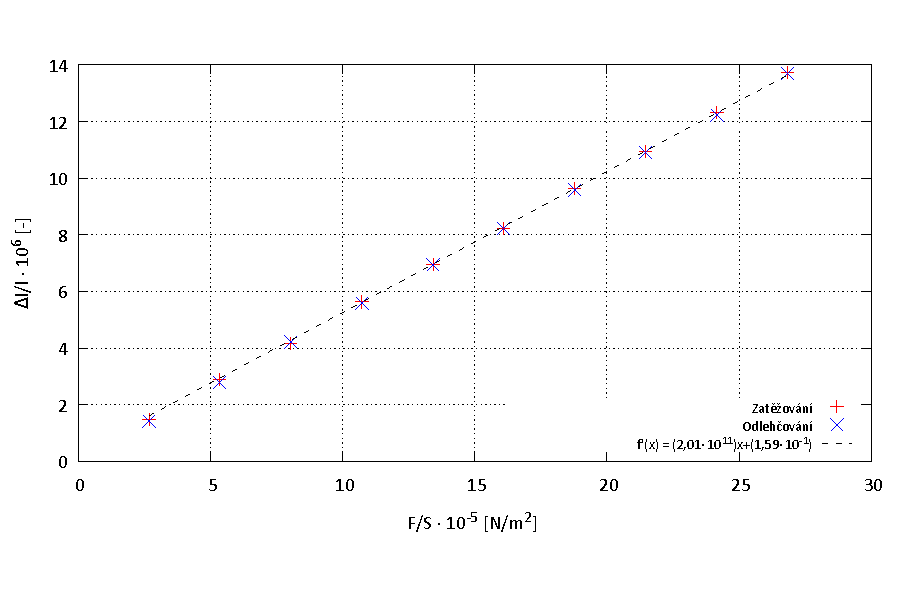
\includegraphics[width=\linewidth]{../gnuplot/data_f1.pdf}
	    \vspace*{-1.5cm}
	    	\caption{Graf závislosti relativního délkového prodloužení $\Delta l/l$ na napětí $F/S$ při zatěžování a odlehčování drátu. Proloženo funkcí inverzní k $f(x) = ax+b$ s druhou řadou parametrů získaných z metody nejmenších čtverců.}
			\label{fig:f_1}
	\end{center}
	\end{figure}

% Table generated by Excel2LaTeX from sheet 'List1'
\begin{table}[h!]
  \centering
       \begin{tabular}{|r|r|r|r|r|r|r|r|}
       \hline
       $m$ [g] & $\sigma_m$ [g] & $F\unit{\ [N]}$ & $\sigma_{F}\unit{\ [N]}$ & $z_1$ [mm] & $\sigma_{z_1}$ [mm] & $z_2$ [mm] & $\sigma_{z_2}$ [mm] \bigstrut\\
       \hline
       100,68 & 0,02  & 0,9738 & 0,0002 & 0,28  & 0,01  & 0,29  & 0,01 \bigstrut\\
       \hline
       200,98 & 0,03  & 1,9440 & 0,0003 & 0,52  & 0,01  & 0,54  & 0,01 \bigstrut\\
       \hline
       301,84 & 0,03  & 2,9196 & 0,0003 & 0,76  & 0,01  & 0,78  & 0,01 \bigstrut\\
       \hline
       402,70 & 0,04  & 3,8952 & 0,0004 & 1,01  & 0,01  & 1,02  & 0,01 \bigstrut\\
       \hline
       503,54 & 0,04  & 4,8706 & 0,0004 & 1,27  & 0,01  & 1,28  & 0,01 \bigstrut\\
       \hline
       603,90 & 0,05  & 5,8413 & 0,0005 & 1,51  & 0,01  & 1,53  & 0,01 \bigstrut\\
       \hline
       704,72 & 0,05  & 6,8165 & 0,0005 & 1,75  & 0,01  & 1,77  & 0,01 \bigstrut\\
       \hline
       805,56 & 0,06  & 7,7919 & 0,0006 & 2,00  & 0,01  & 2,01  & 0,01 \bigstrut\\
       \hline
       906,64 & 0,06  & 8,7696 & 0,0006 & 2,23  & 0,01  & 2,25  & 0,01 \bigstrut\\
       \hline
       \end{tabular}%
 \caption{Naměřené a spočítané hodnoty při měření modulu pružnosti v tahu \emph{E} z průhybu nosníku: $m$ a $\sigma_m$ jsou celková hmotnost zavěšených závaží s chybou, $F$ a $\sigma_{F}$ síla působící na nosník a její chyba (\ref{eq:chyba_neprime_mereni}), $z_{1,2}$ průhyb nosníku při zatěžování a odlehčování v jeho středu a $\sigma_{z_{1,2}}$ jejich chyby (\ref{eq:chyba_neprime_mereni}) . }
 \label{tab:E2}%
\end{table}%
	
		\begin{figure}[h!]
		\begin{center}
		\vspace*{-1.5cm}
		    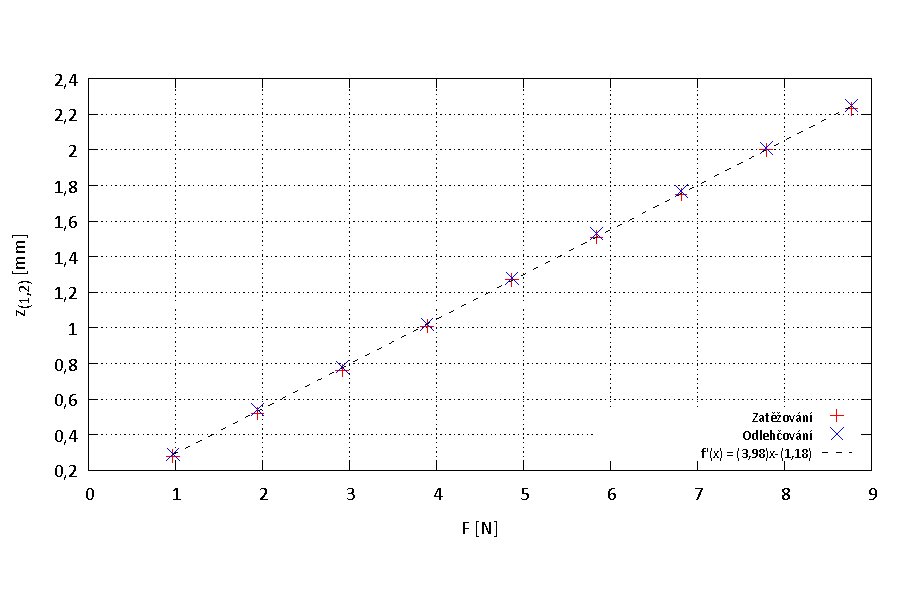
\includegraphics[width=\linewidth]{../gnuplot/data_f2.pdf}
		    \vspace*{-1.5cm}
		    	\caption{Graf závislosti průhybu nosníku $z_{(1,2)}$ na síle $F$ působící v jejím středu při zatěžování a odlehčování. Proloženo funkcí inverzní k $f(x) = ax+b$ s druhou řadou parametrů získaných z metody nejmenších čtverců.}
				\label{fig:f_2}
		\end{center}
		\end{figure}

% Table generated by Excel2LaTeX from sheet 'List1'
\begin{table}[htbp]
  \centering
	       \begin{tabular}{|r|r|r|r|r|r|r|r|}
           \hline
          $m$ [g] & $\sigma_m$ [g] & $M\unit{\ [N\cdot m]}$ & $\sigma_{M}\unit{\ [N\cdot m]}$ & $\Delta \varphi_1 \unit{\ [^\circ] }$  & $\sigma_{\Delta \varphi_1 } \unit{\ [^\circ] }$ & $\Delta \varphi_2 \unit{\ [^\circ] }$  & $\sigma_{\Delta \varphi_2 } \unit{\ [^\circ] }$ \bigstrut\\
              \hline
           201,64 & 0,03  & 0,0401 & 0,0002 & 10,0  & 0,5   & 9,5   & 0,5 \bigstrut\\
           \hline
           403,36 & 0,04  & 0,0801 & 0,0004 & 24,0  & 0,5   & 23,5  & 0,5 \bigstrut\\
           \hline
           605,04 & 0,05  & 0,1202 & 0,0006 & 32,5  & 0,5   & 33,5  & 0,5 \bigstrut\\
           \hline
           805,76 & 0,06  & 0,1601 & 0,0008 & 44,5  & 0,5   & 45,5  & 0,5 \bigstrut\\
           \hline
           1008,02 & 0,06  & 0,2000 & 0,0010 & 54,5  & 0,5   & 54,5  & 0,5 \bigstrut\\
           \hline
           1209,00 & 0,07  & 0,2400 & 0,0010 & 61,5  & 0,5   & 61,5  & 0,5 \bigstrut\\
           \hline
           \end{tabular}%             
 \caption{Naměřené a spočítané hodnoty při měření modulu pružnosti ve smyku \emph{G} torzí drátu statickou metodou: $m$ a $\sigma_m$ jsou celková hmotnost zavěšených závaží s chybou, $M$ a $\sigma_{M}$ moment sil tvořený závažími a jeho chyba (\ref{eq:chyba_neprime_mereni}), $\Delta \varphi_{1,2}$ úhly torze odečtené z úhloměru a $\sigma_{\Delta \varphi_{1,2}}$ jejich chyby. }
 \label{tab:G1}%
\end{table}%

	\begin{figure}[h!]
	\begin{center}
	\vspace*{-1.5cm}
	    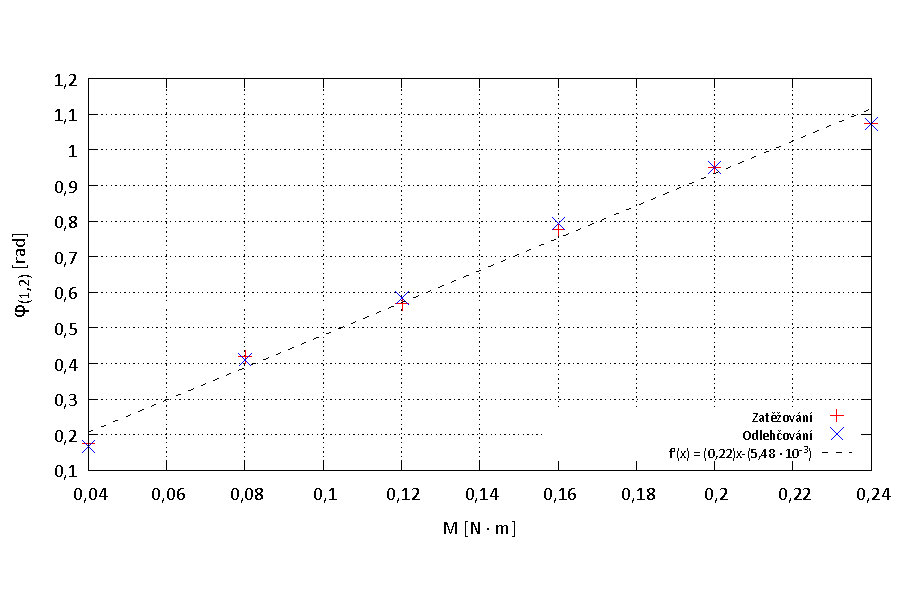
\includegraphics[width=\linewidth]{../gnuplot/data_g1.pdf}
	    \vspace*{-1.5cm}
	    	\caption{Graf závislosti změny torzního úhlu $\Delta \varphi_{(1,2)}$ na silovém momentu $M$ působícím vlivem dvou sad závaží při zatěžování a odlehčování. Proloženo funkcí inverzní k $f(x) = ax+b$ s druhou řadou parametrů získaných z metody nejmenších čtverců.}
			\label{fig:g_1}
	\end{center}
	\end{figure}

\clearpage
% Table generated by Excel2LaTeX from sheet 'List1'
\begin{table}[htbp]
  \centering
	       \begin{tabular}{|r|r|r|r|}
	           \hline
	           $T_1$ [s] & $\sigma_{T_1}$ [s] & $T_0$ [s] & $\sigma_{T_0}$ [s] \bigstrut\\
	           \hline
	           13,3  & 0,1   & 4,3   & 0,1 \bigstrut\\
	           \hline
	           13,3  & 0,1   & 4,3   & 0,1 \bigstrut\\
	           \hline
	           13,3  & 0,1   & 4,3   & 0,1 \bigstrut\\
	           \hline
	           13,2  & 0,1   & 4,3   & 0,1 \bigstrut\\
	           \hline
	           13,3  & 0,1   & 4,3   & 0,1 \bigstrut\\
	           \hline
	           13,3  & 0,1   & 4,3   & 0,1 \bigstrut\\
	           \hline
	           13,3  & 0,1   & 4,3   & 0,1 \bigstrut\\
	           \hline
	           13,3  & 0,1   & 4,3   & 0,1 \bigstrut\\
	           \hline
	           13,3  & 0,1   & 4,3   & 0,1 \bigstrut\\
	           \hline
	           13,3  & 0,1   & 4,3   & 0,1 \bigstrut\\
	           \hline
	           13,3  & 0,1   & 4,3   & 0,1 \bigstrut\\
	           \hline
	           \end{tabular}%
	                 
 \caption{Spočítané hodnoty při měření modulu pružnosti ve smyku \emph{G} torzí drátu dynamickou metodou: $T_1$ a $\sigma_{T_1}$ jsou periody získané postupnou metodou (z deseti různých intervalů deseti period) s příslušnou chybou (\ref{eq:chyba_aritmetickeho_prumeru}) při kmitání tyče s velkými disky na okrajích, $T_0$ a $\sigma_{T_0}$ pak analogicky pro kmitání samotné tyče.}
 \label{tab:G2}%
\end{table}%

	\begin{figure}[h!]
	\centering
	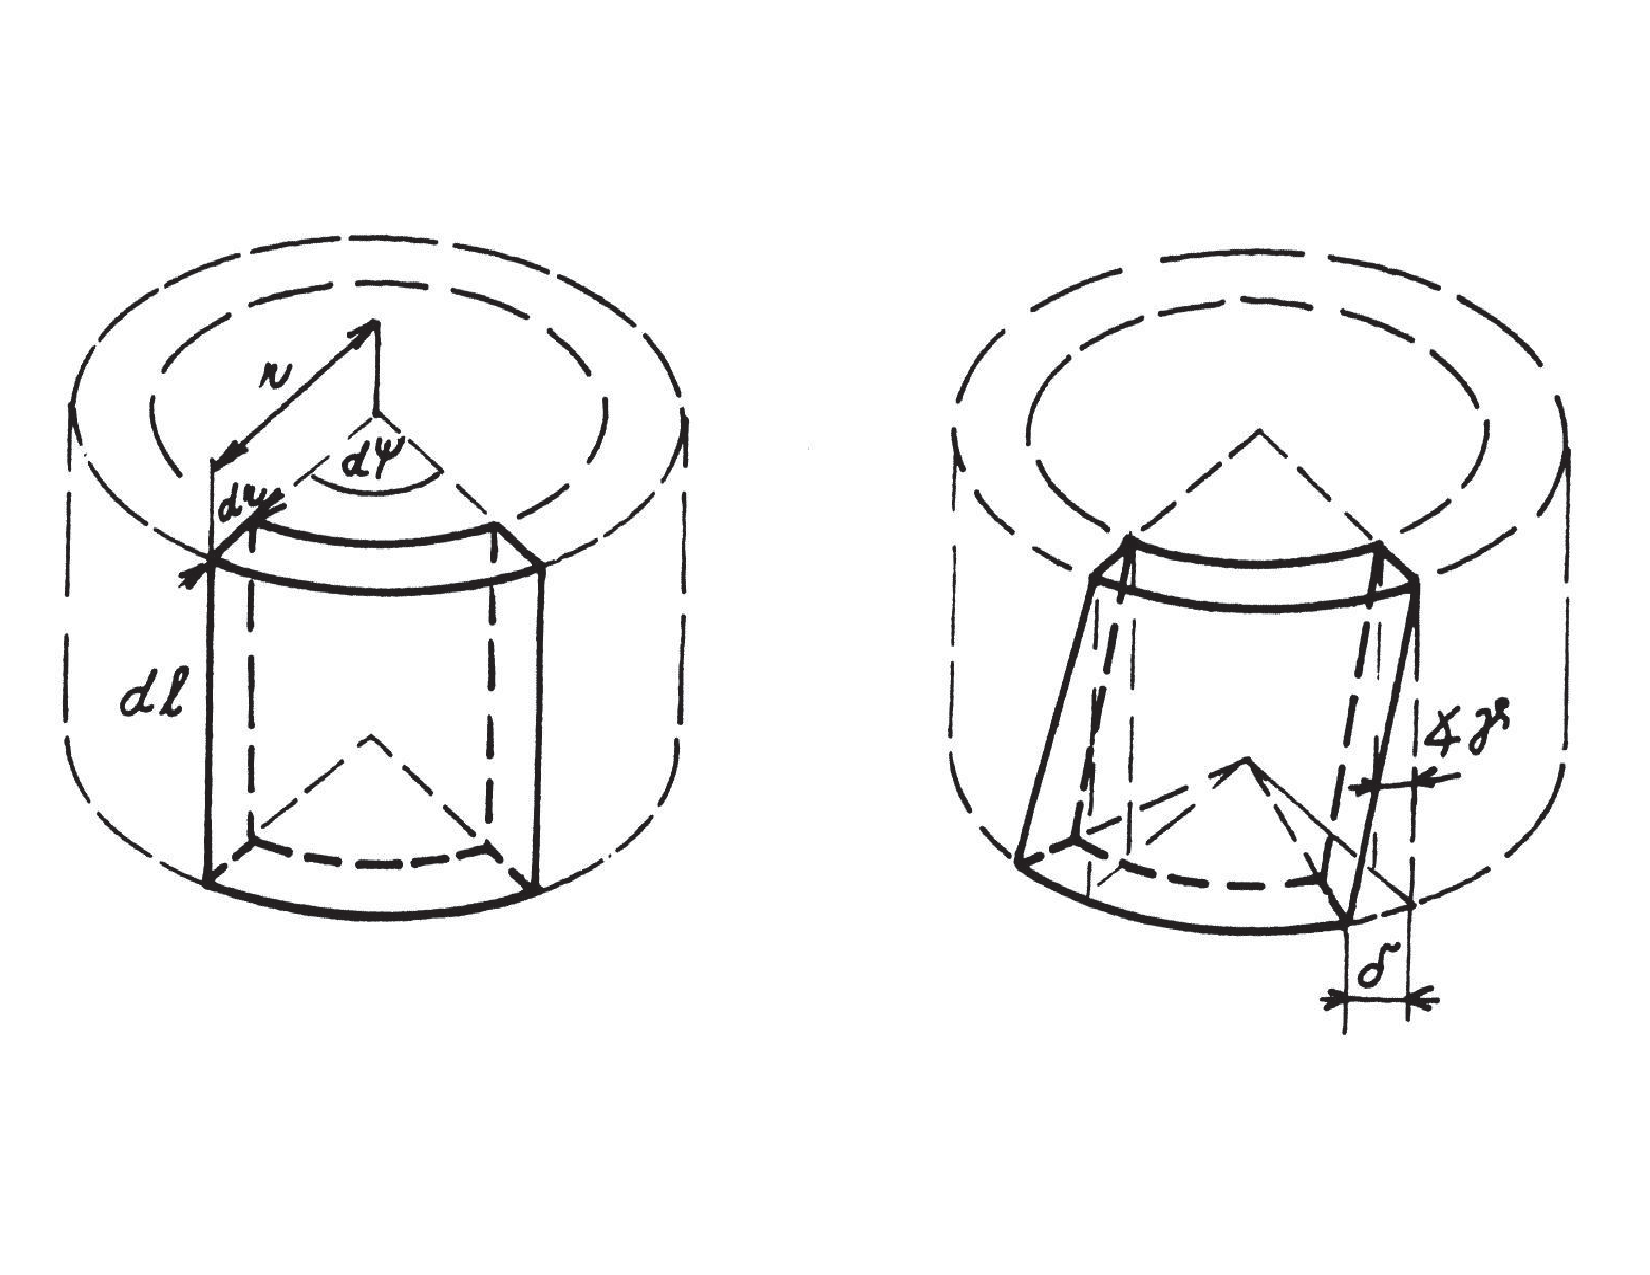
\includegraphics[width=10cm]{att/torze_element.pdf}
	\vspace*{-2cm}
	\caption{Smyk elementárního hranolu vyříznutého z válce při torzi \cite{bib:zadani}}
	\label{fig:torze_element}
	\end{figure}

\clearpage
\subsection{Schémata}

	\begin{figure}[h!]
	\centering
	\begin{minipage}{.45\textwidth}
	  \centering
					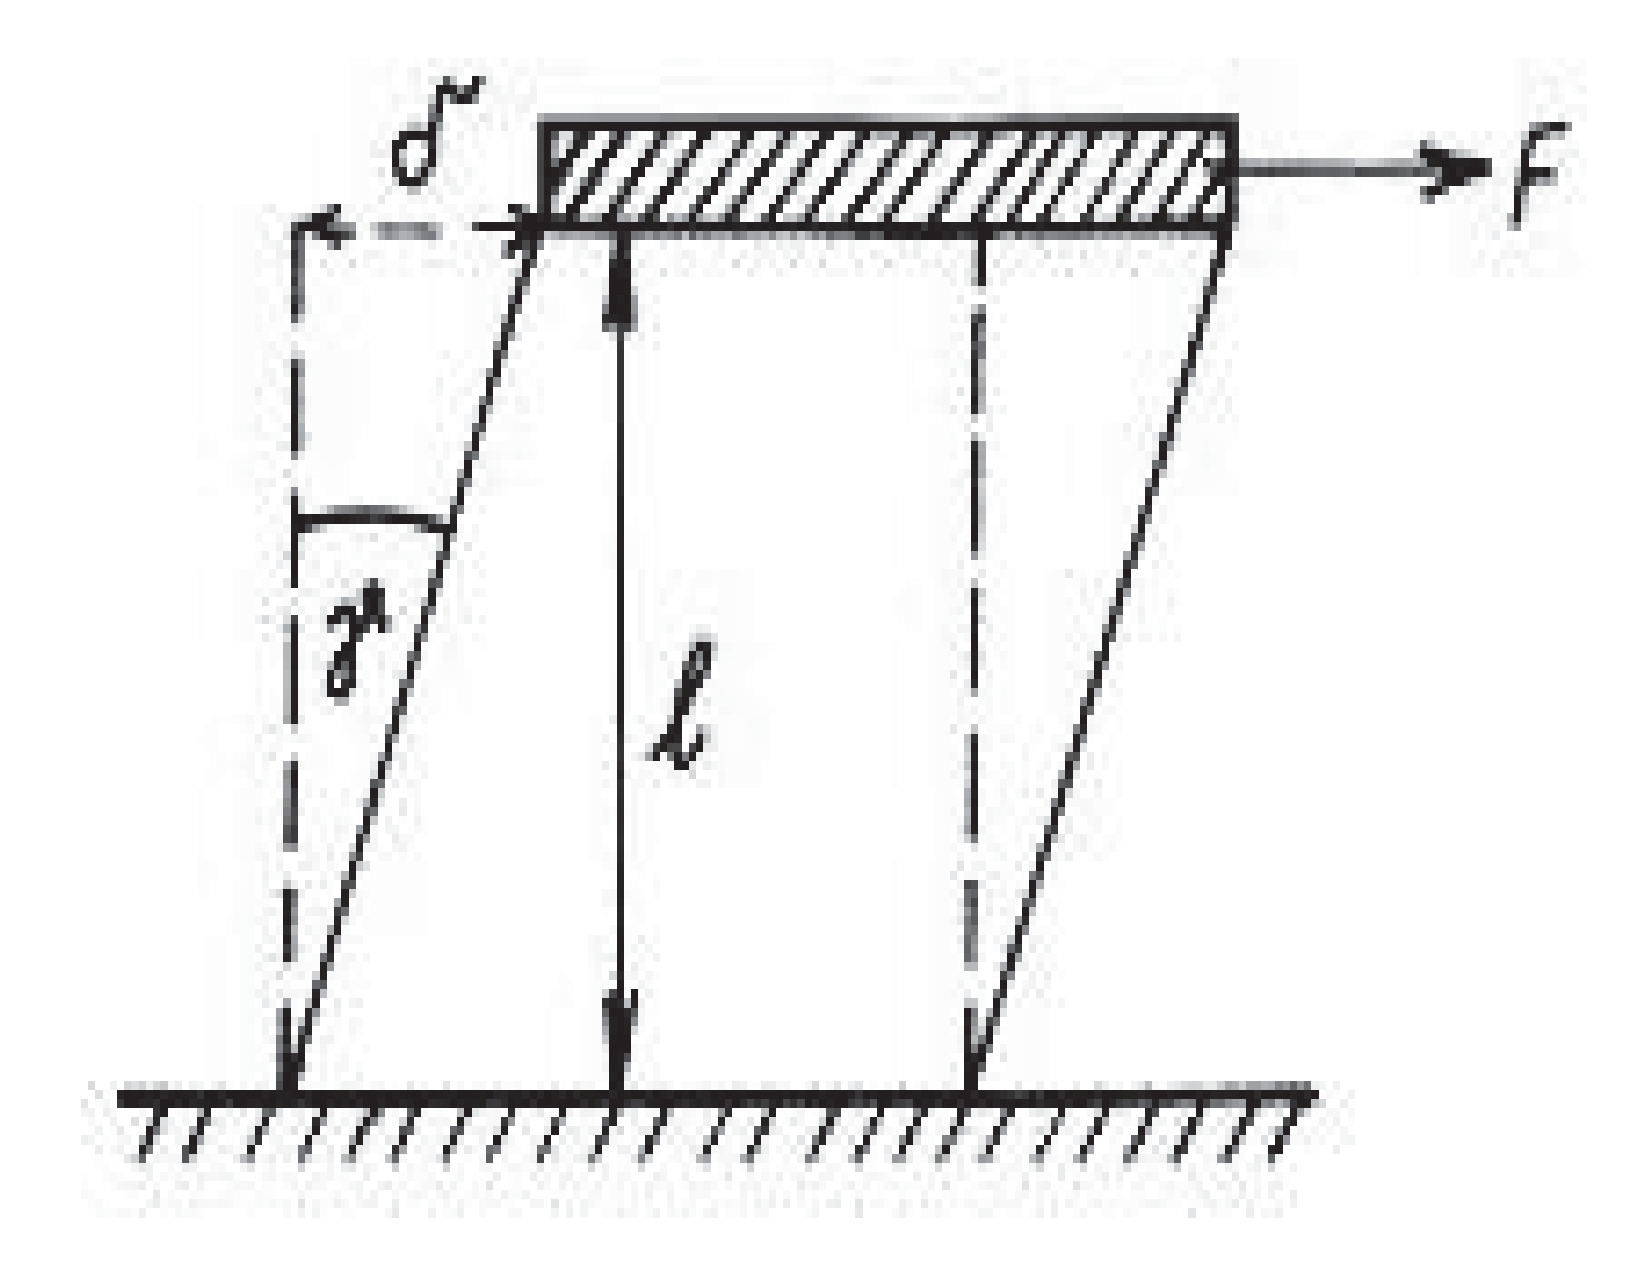
\includegraphics[width=5cm]{att/smyk.pdf}
					\caption{Schéma smyku \cite{bib:zadani}}
					\label{fig:s_smyk}
	\end{minipage}%
	\hfill
	\begin{minipage}{.45\textwidth}
	  \centering
					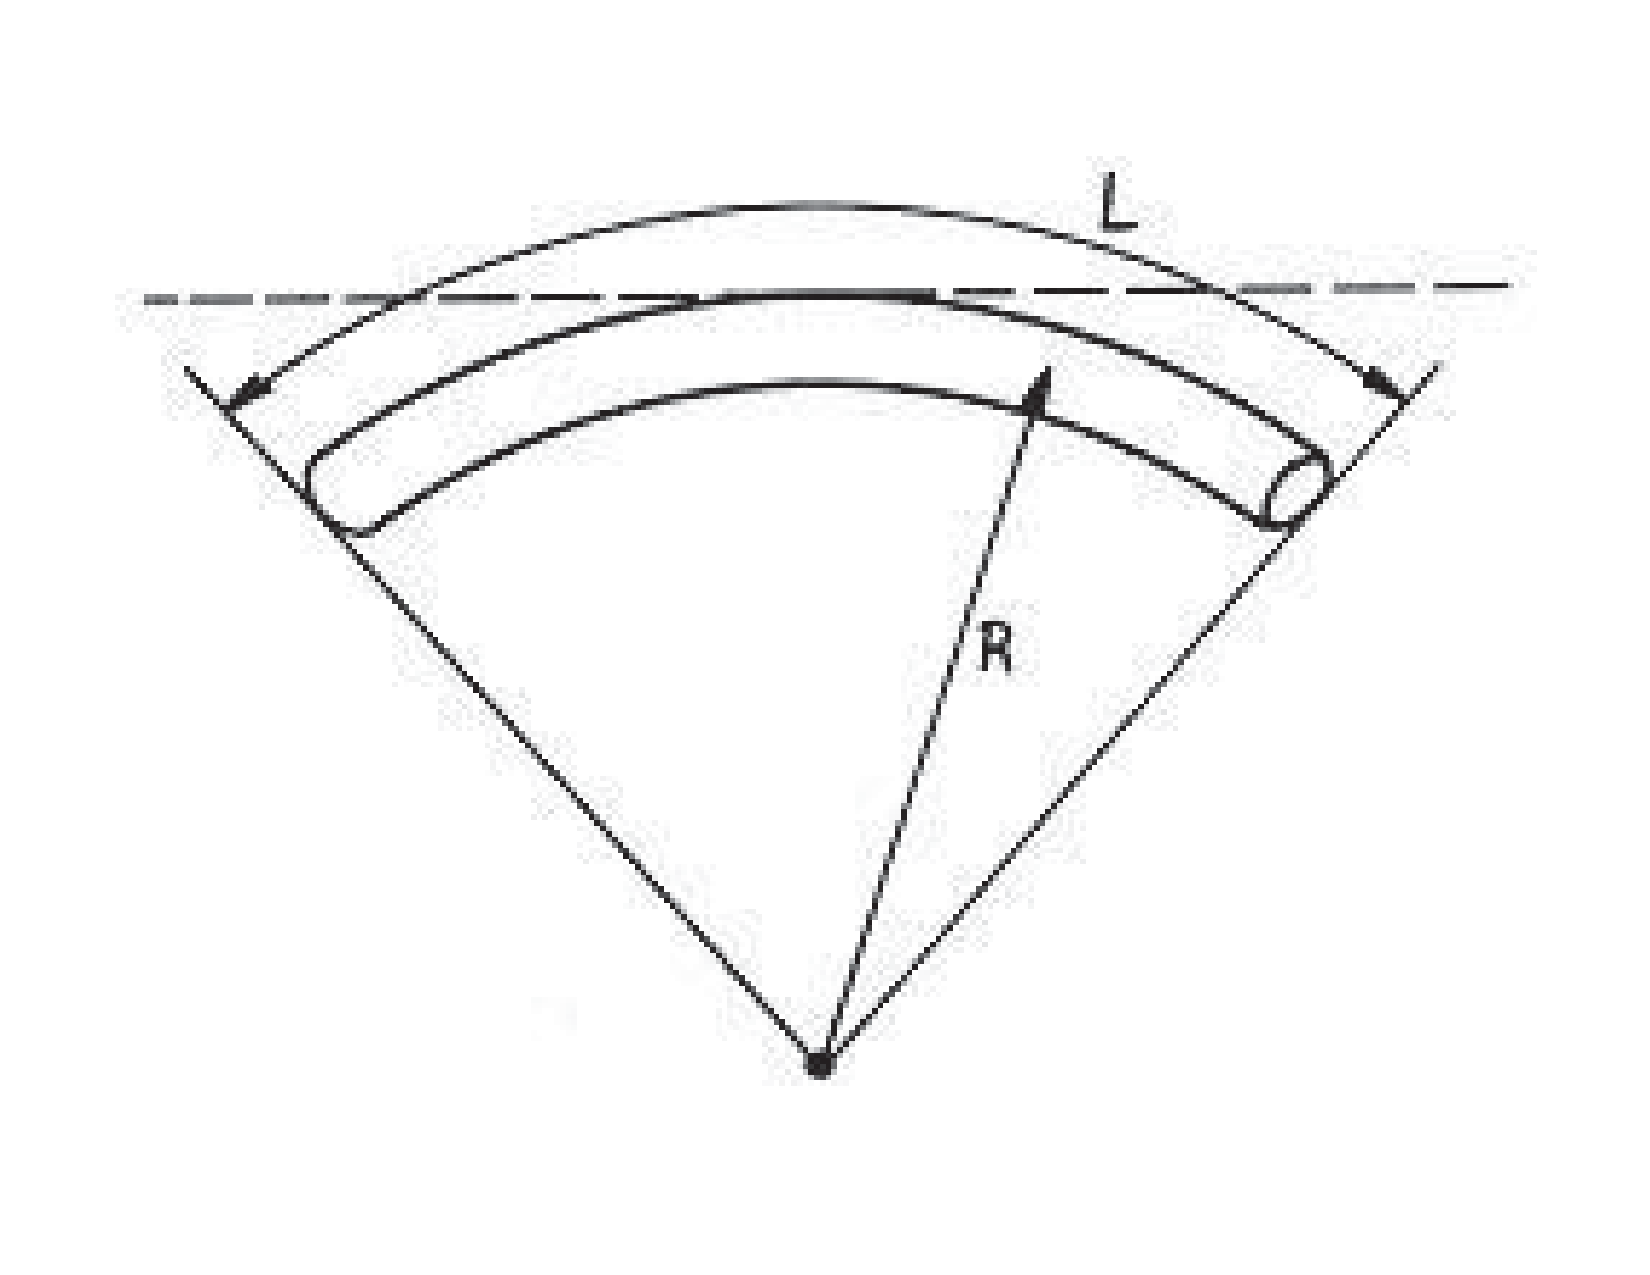
\includegraphics[width=5cm]{att/ohyb_nosniku.pdf}
					\caption{Ohyb nosníku \cite{bib:zadani}}
					\label{fig:s_ohyb}
	\end{minipage}
	\end{figure}

	\begin{figure}[h!]
	\centering
	\begin{minipage}{.55\textwidth}
	  \centering
					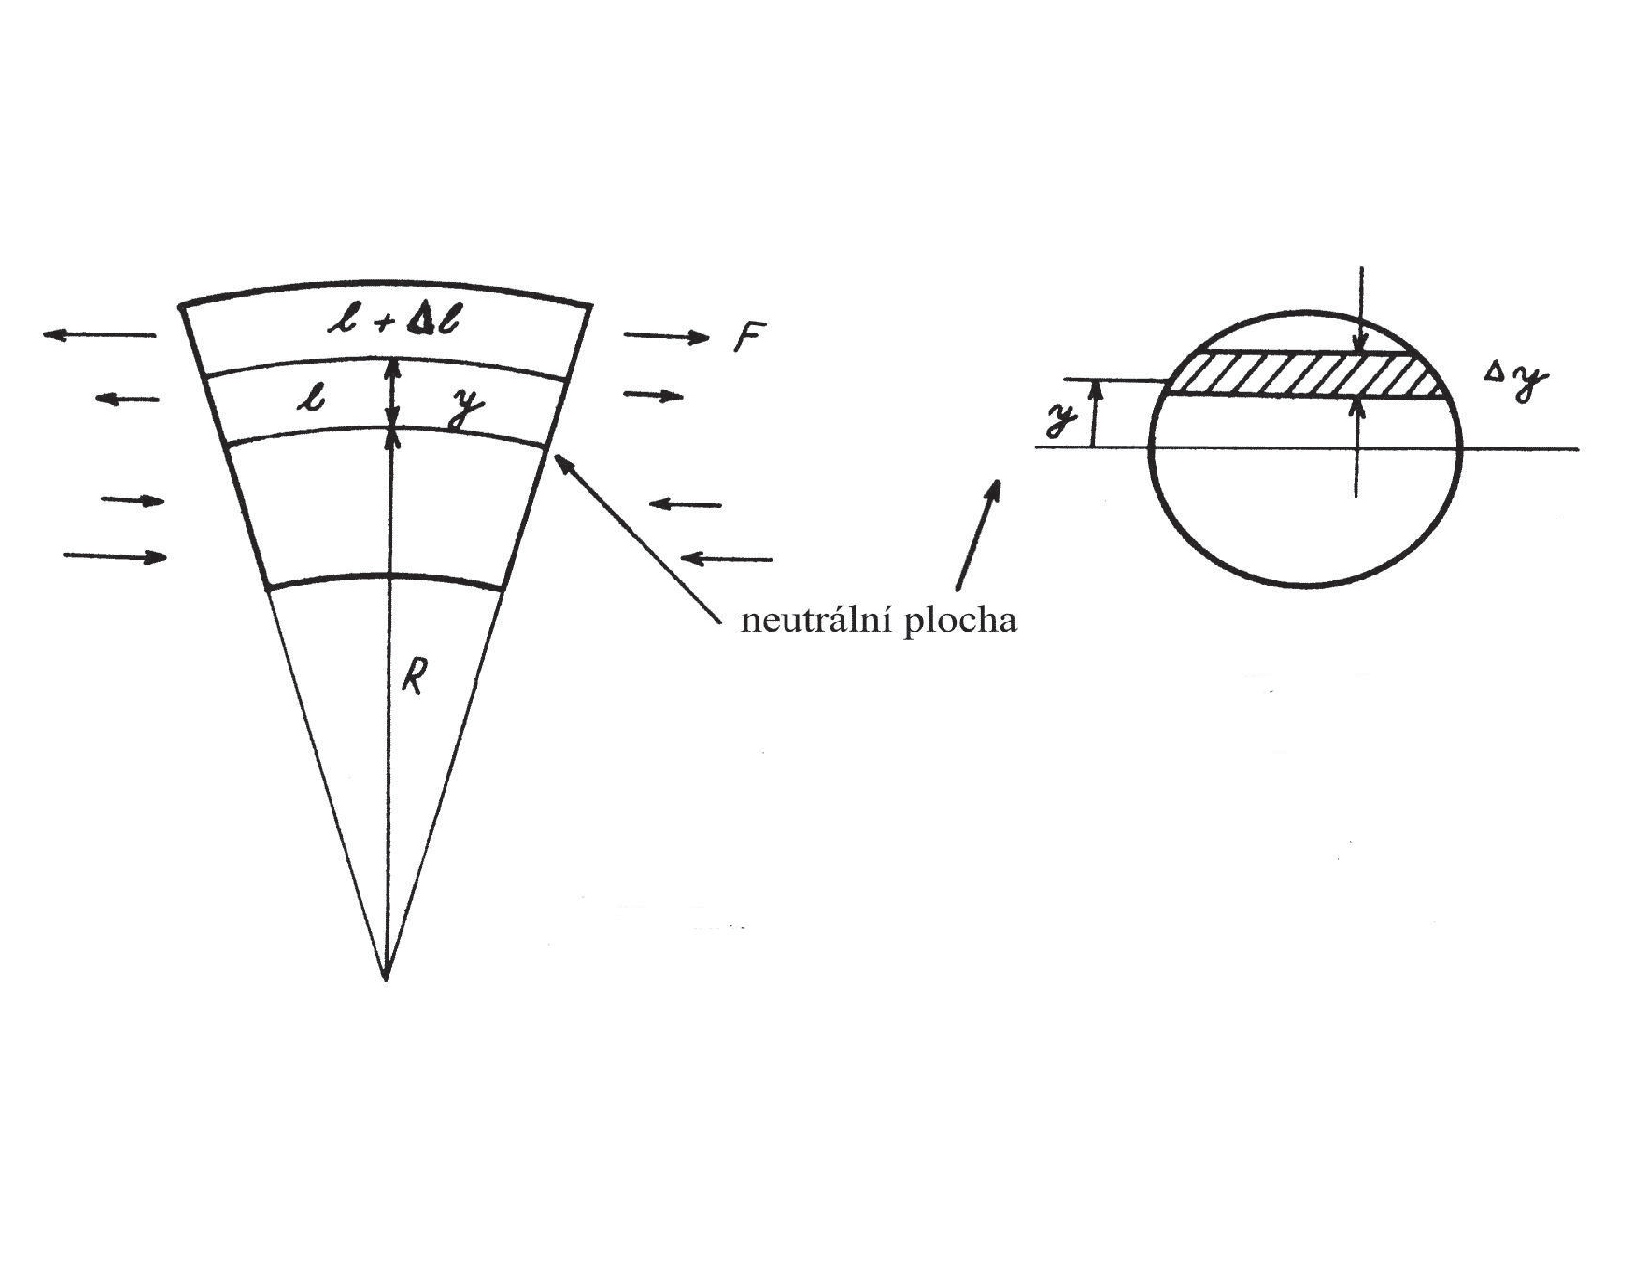
\includegraphics[width=9cm]{att/neutralni_plocha.pdf}
					\vspace*{-1.5cm}
					\caption{Neutrální plocha, deformace nosníku při ohybu \cite{bib:zadani}}
					\label{fig:s_neutralniplocha}
	\end{minipage}%
	\hfill
	\begin{minipage}{.35\textwidth}
	  \centering
					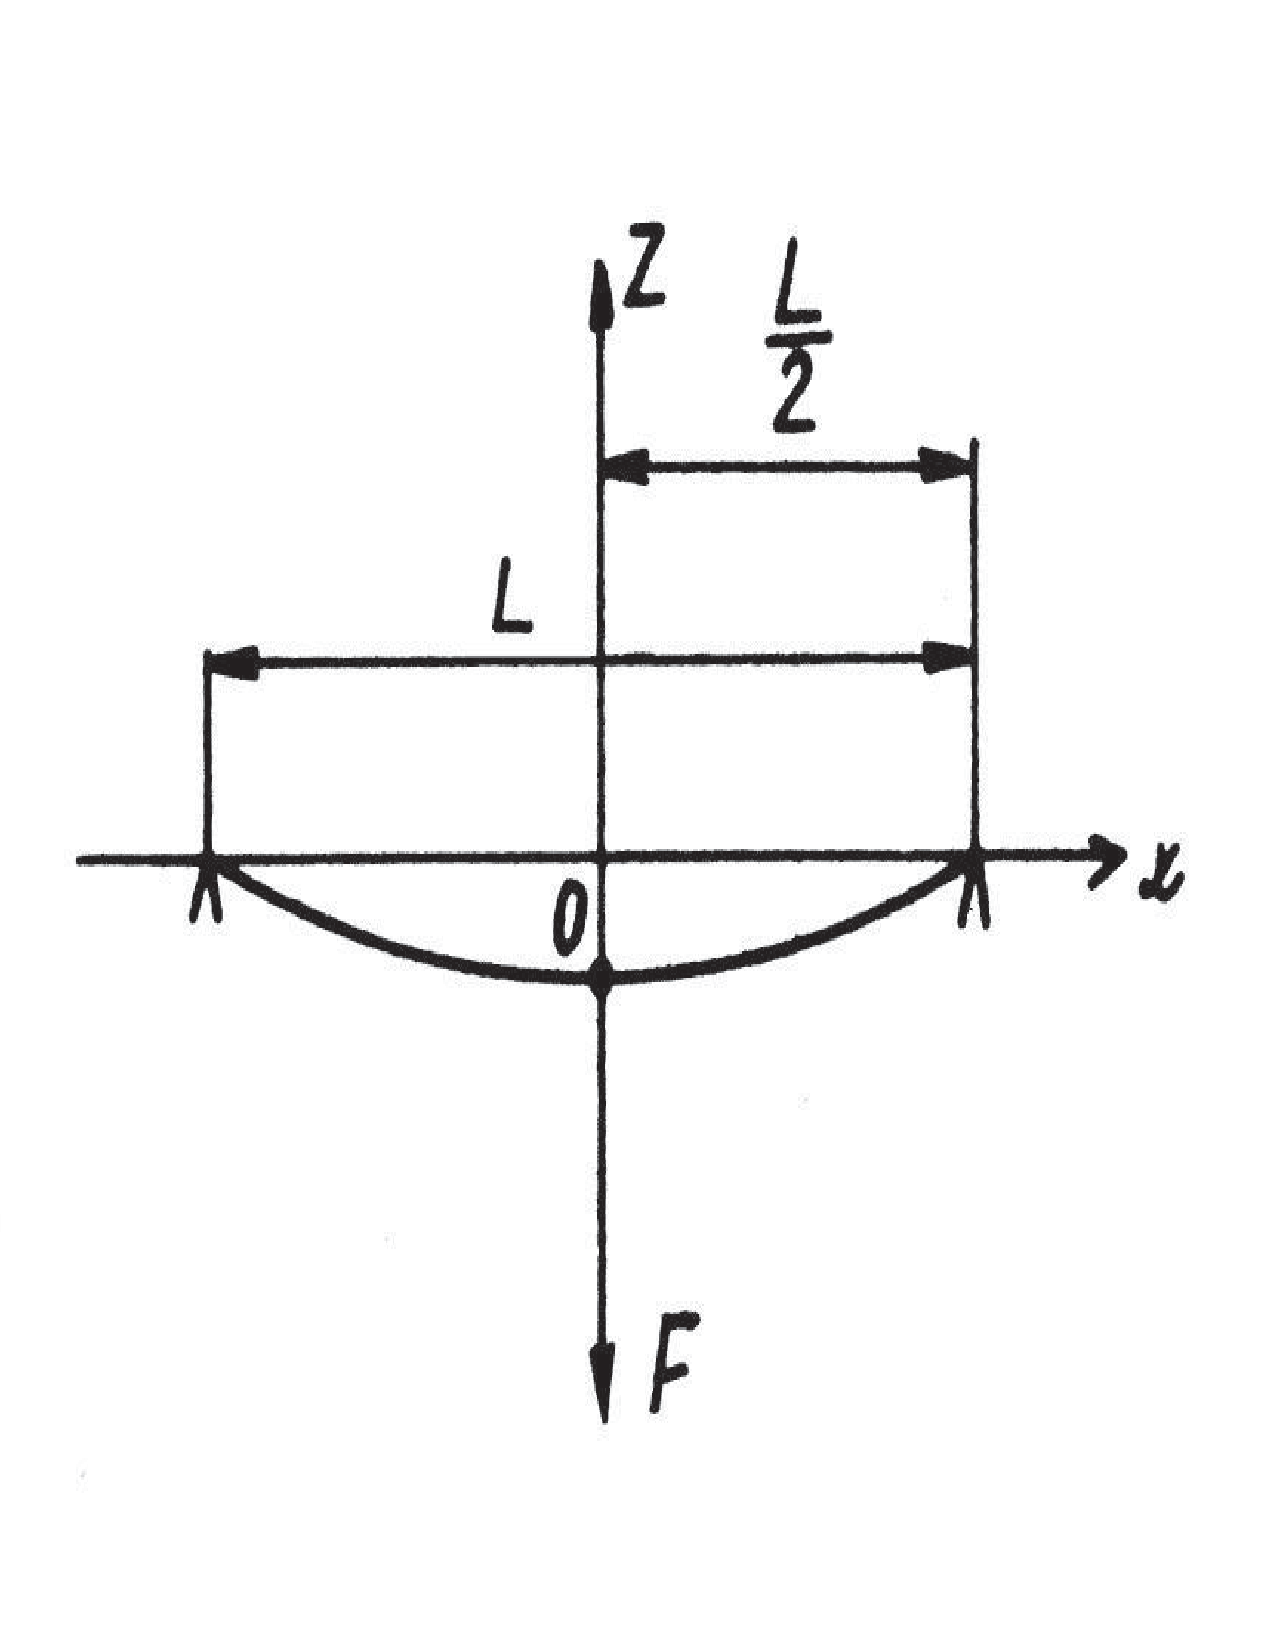
\includegraphics[width=5cm]{att/ohyb_priklad.pdf}
					\vspace*{-0.5cm}
					\caption{Ohyb nosníku podepřeného na břitech \cite{bib:zadani}}
					\label{fig:s_ohyb_priklad}
	\end{minipage}
	\end{figure}

	\begin{figure}[h!]
	\centering
	\begin{minipage}{.30\textwidth}
	  \centering
					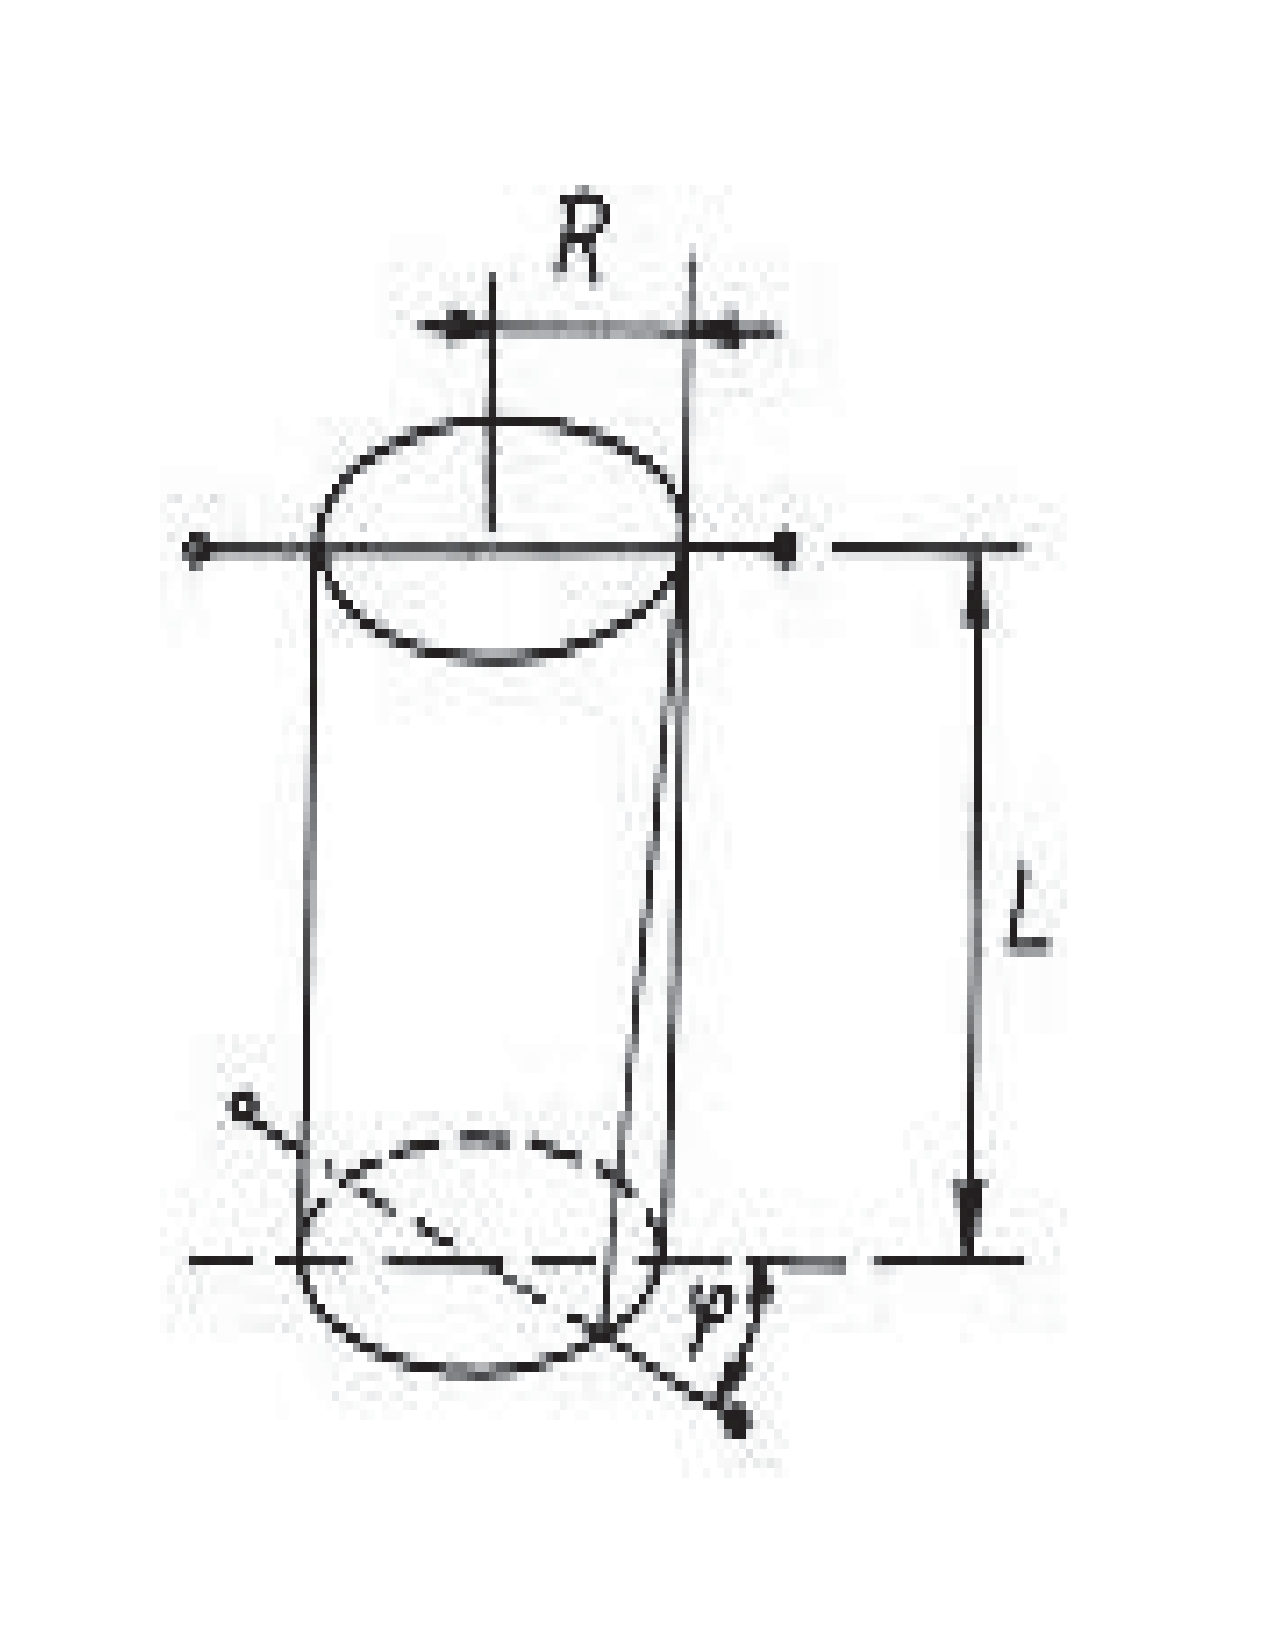
\includegraphics[width=5cm]{att/torze_valce.pdf}
					\vspace*{-0.5cm}
					\caption{Torze válce kruhového průřezu \cite{bib:zadani}}
					\label{fig:torze_valce}
	\end{minipage}%
	\hfill
	\begin{minipage}{.30\textwidth}
	  \centering
					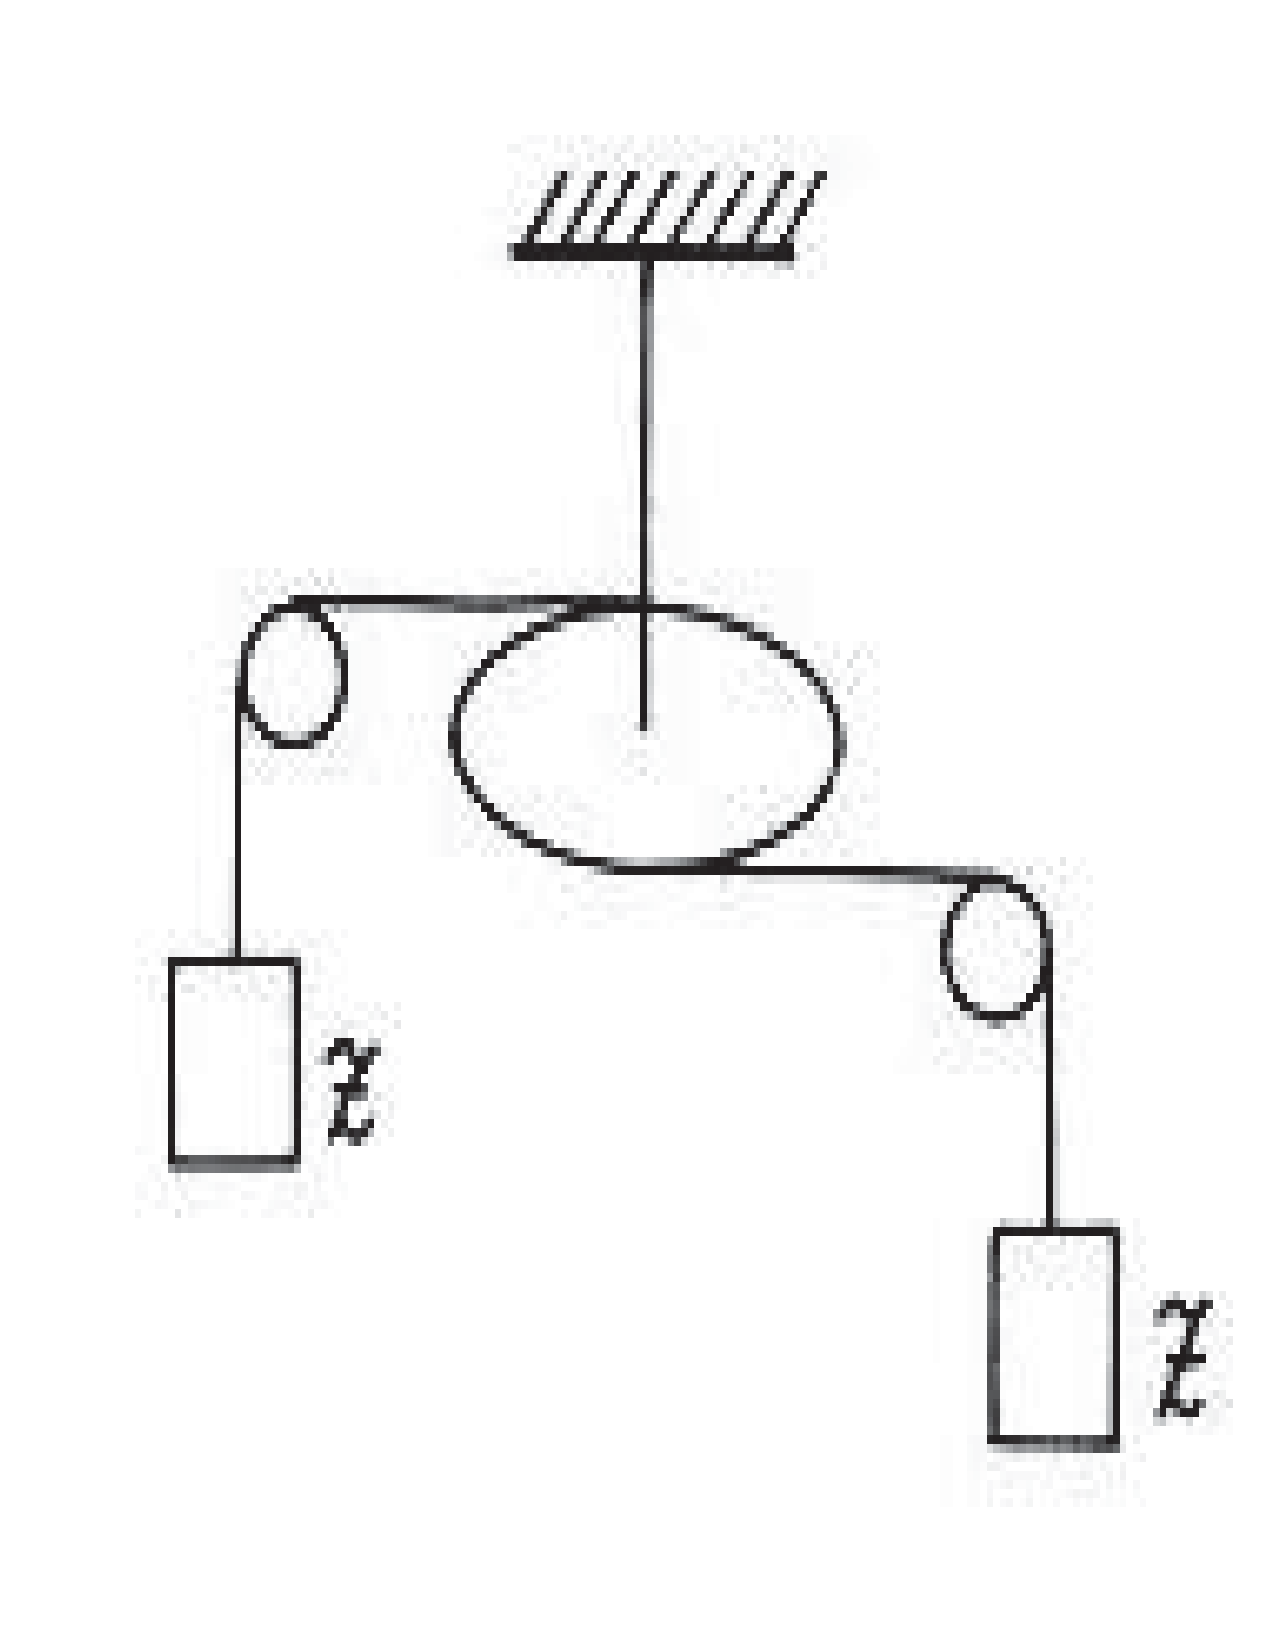
\includegraphics[width=5cm]{att/torze_staticka.pdf}
					\vspace*{-0.5cm}
					\caption{Zařízení pro měření modulu pružnosti ve smyku statickou metodou \cite{bib:zadani}}
					\label{fig:torze_staticka}
	\end{minipage}
	\hfill
	\begin{minipage}{.30\textwidth}
	  \centering
					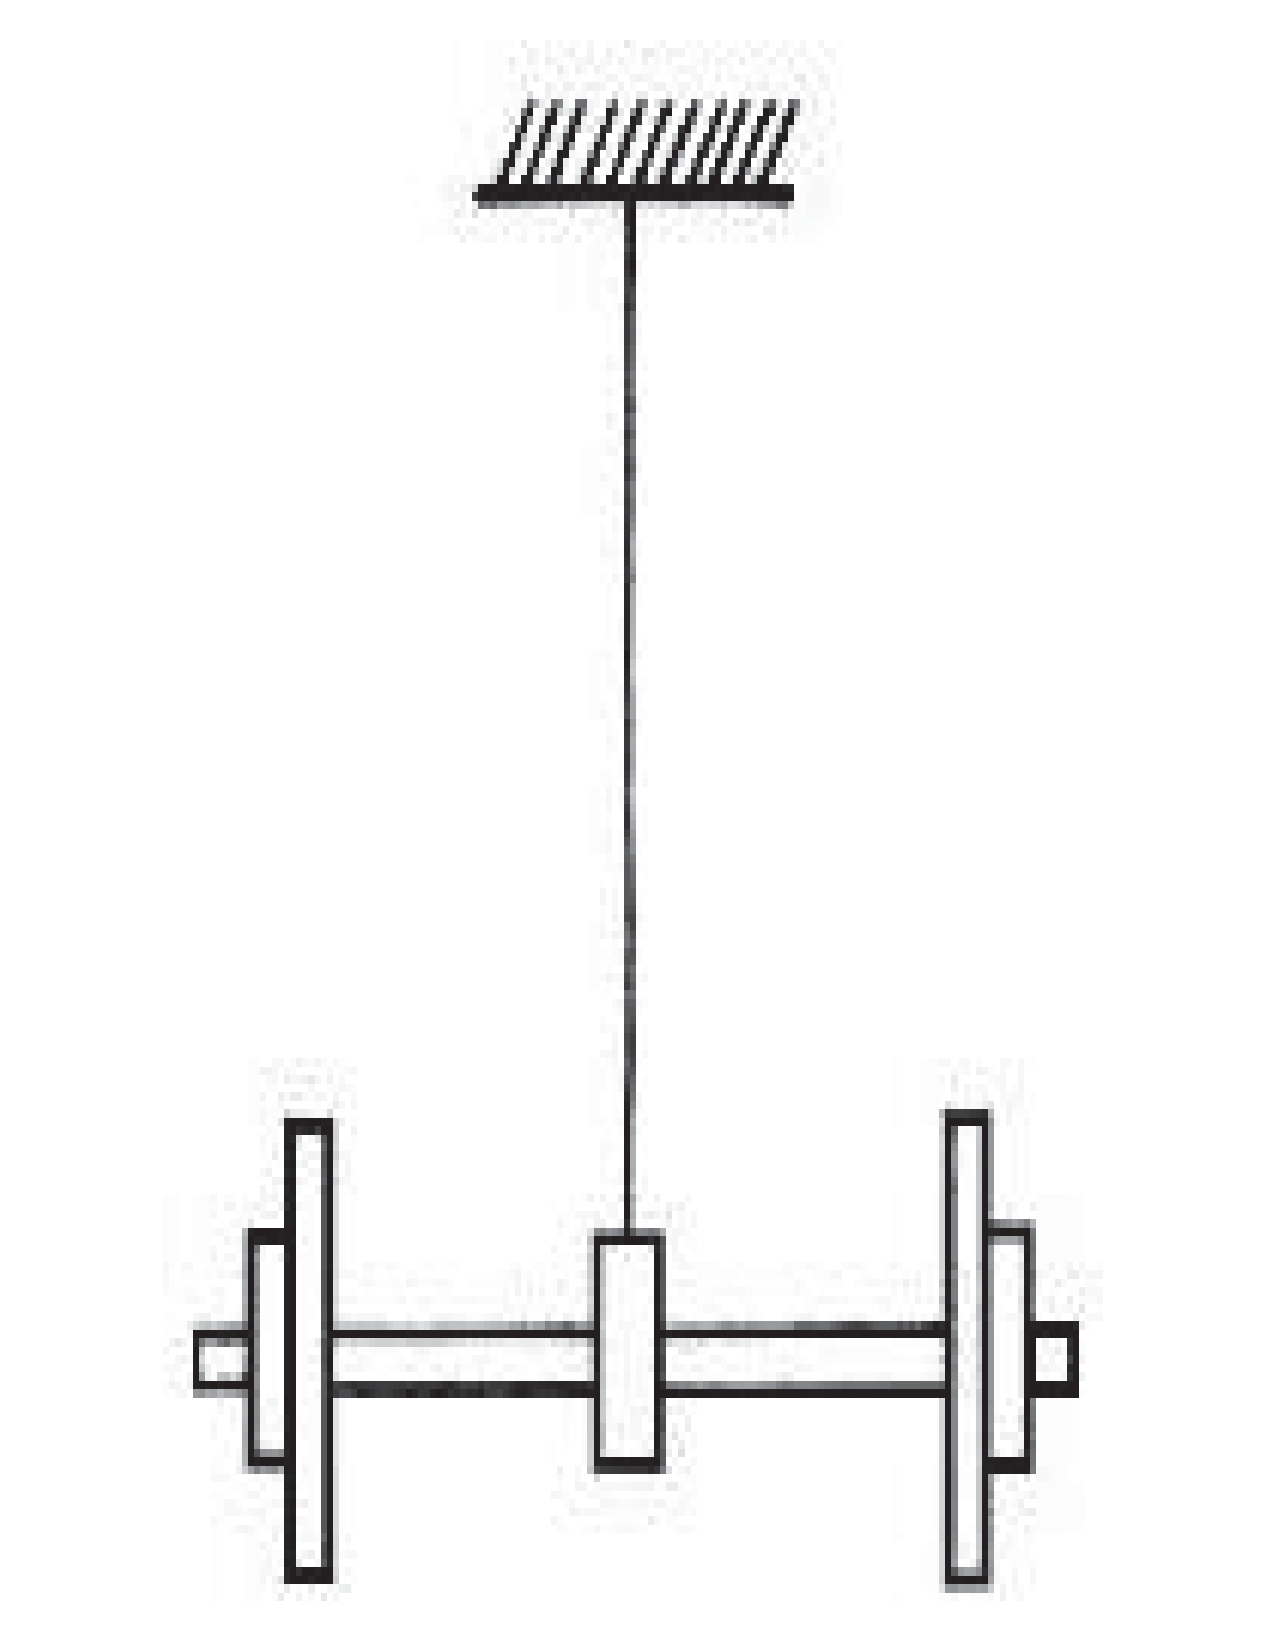
\includegraphics[width=5cm]{att/torze_dynamicka.pdf}
					\caption{Zařízení pro měření modulu pružnosti ve smyku dynamickou metodou \cite{bib:zadani}}
					\label{fig:torze_dynamicka}
	\end{minipage}
	\end{figure}
				
\clearpage
	
% --- Konec dokumentu --------------------------------------------------


\end{document}

